\documentclass[oneside]{estilo}

% Importações de pacotes
\usepackage[alf, abnt-emphasize=bf, recuo=0cm, abnt-etal-cite=2, abnt-etal-list=0]{abntex2cite}  % Citações padrão ABNT
\usepackage[utf8]{inputenc}                         % Acentuação direta
\usepackage[T1]{fontenc}                            % Codificação da fonte em 8 bits
\usepackage{graphicx}                               % Inserir figuras
\usepackage{amsfonts, amssymb, amsmath}             % Fonte e símbolos matemáticos
\usepackage{booktabs}                               % Comandos para tabelas
\usepackage{verbatim}                               % Texto é interpretado como escrito no documento
\usepackage{multirow, array}                        % Múltiplas linhas e colunas em tabelas
\usepackage{indentfirst}                            % Endenta o primeiro parágrafo de cada seção.
\usepackage{microtype}                              % Para melhorias de justificação
\usepackage[algoruled, portuguese]{algorithm2e}     % Escrever algoritmos
\usepackage{float}                                  % Utilizado para criação de floats
%\usepackage{times}                                 % Usa a fonte Times

\usepackage{color}
\usepackage{chronosys}
\usepackage{pdflscape}
%\usepackage{tabu}
\usepackage{makecell}
\usepackage{nameref}
\usepackage{listings}
\usepackage{enumitem}
\usepackage{chngcntr}
\usepackage{colortbl}
\usepackage[htt]{hyphenat}
\usepackage{mdframed}

\mdfsetup{skipabove=1.5\topskip,skipbelow=0.5\topskip}
\mdfdefinestyle{pp}{%
	linecolor=black,
	outerlinewidth=.5pt,
	roundcorner=5pt,
	innertopmargin=8pt,
	innerbottommargin=0.5\baselineskip,
	usetwoside=false
}

%\usepackage{minitoc}
%\dominitoc% Initialization
\newcommand{\enumerateletter}[2]{\textbf{#1\textsubscript{#2}}}

% Inclui o preâmbulo do documento
%
% Documento: Preâmbulo + Capa
%

% -------------------------------
% Pacotes necessários
% -------------------------------
\usepackage{lmodern}     % Fonte Latin Modern
\usepackage{listings}    % Ambientes de código
\usepackage{tocloft}     % Personalização das listas
\usepackage{chngcntr}    % Necessário para \counterwithin

% -------------------------------
% Configuração de listagens
% -------------------------------
\renewcommand{\lstlistingname}{Código}

\counterwithin{figure}{chapter}
\counterwithin{table}{chapter}

% Criação da "Lista de Códigos" conforme ABNT
\begingroup\makeatletter
\let\newcounter\@gobble
\let\setcounter\@gobbletwo
\globaldefs\@ne
\let\c@loldepth\@ne
\newlistof{listings}{lol}{\lstlistlistingname}
\newlistentry{lstlisting}{lol}{0}
\endgroup

\renewcommand{\cftlstlistingaftersnum}{\hfill--\hfill}

\let\oldlstlistoflistings\lstlistoflistings
\renewcommand{\lstlistoflistings}{%
  \begingroup%
  \let\oldnumberline\numberline%
  \renewcommand{\numberline}{\lstlistingname\space\oldnumberline}%
  \oldlstlistoflistings%
  \endgroup}

% Estilo para códigos
\lstdefinestyle{master-thesis}{
  basicstyle=\ttfamily\small,
  numbers=left,
  numberstyle=\tiny,
  frame=tb,
  columns=fullflexible,
  showstringspaces=false,
  captionpos=b,
  breaklines=true,
  tabsize=2
}
\lstset{style=master-thesis}

% -------------------------------
% ==== DADOS DA CAPA (ÚNICO LUGAR PARA EDITAR) ====


\instituicao{UNIFIO - CENTRO UNIVERSITÁRIO DE OURINHOS}
\departamento{CURSO: ENGENHARIA DE SOFTWARE}
\titulotb{SISTEMA DE APOIO A PROFESSORES DO ENSINO FUNDAMENTAL PARA CRIAÇÃO DE ATIVIDADES ADAPTADAS A CRIANÇAS NEURODIVERGENTES}

\nomeautor{%
  \textbf{EDSON CARLOS VICENTIM JUNIOR}\\
  \textbf{MIGUEL ANGELO BURATI MORALEZ}\\
  \textbf{PEDRO HENRIQUE SILVÉRIO DA FONSECA}\\
  \textbf{VICTOR AUGUSTO MOREIRA BARBOSA}%
}

\localapresentacao{Ourinhos -- São Paulo}
\anoapresentacao{2026}


\usepackage[a4paper, top=3.0cm, bottom=2.0cm, left=3.0cm, right=2.0cm]{geometry} %teste margem

\newcommand{\blue}[1]{\textcolor{blue}{#1}} % proposed
\newcommand{\red}[1]{\textcolor{red}{#1}} % to be removed
\newcommand{\green}[1]{\textcolor{green}{#1}} % to be discussed?
\newcommand{\magenta}[1]{\textcolor{magenta}{#1}} % warning - requires attention

\settocdepth{subsection}

% Define as cores dos links e informações do PDF
\makeatletter
\hypersetup{
    portuguese,
    colorlinks,
    linkcolor=blue,
    citecolor=blue,
    filecolor=black,
    urlcolor=black,
    breaklinks=true,
    pdftitle={\imprimirtitulotb},
    pdfauthor={\imprimirnomeautor}
}
\makeatother

% Redefinição de labels
\renewcommand{\algorithmautorefname}{Algoritmo}
\def\equationautorefname~#1\null{Equa\c c\~ao~(#1)\null}

% Cria o índice remissivo
\makeindex

% Início do documento
\begin{document}

    % Retira espaço extra obsoleto entre as frases.
    \frenchspacing

    % Elementos pré-textuais
    \pretextual
    \include{01-elementos-pre-textuais/dados}       % único lugar onde você edita capa
    %
% Documento: Capa
%

\makeatletter
\begin{capa}
	\thispagestyle{empty}%limpa estilo da pagina
	\setlength{\baselineskip}{0.72\baselineskip}
    \begin{center} %Alinhamento centralizado
	

    \textbf{\expandafter\uppercase\expandafter{\imprimirinstituicao}}\\
    \textbf{\expandafter\uppercase\expandafter{\imprimirdepartamento}}\\
    %\textbf{\expandafter\uppercase\expandafter{\imprimirprograma}}\\
	\vspace*{5cm}%Espaçamento entre linhas
	\large\textbf{\expandafter\uppercase\expandafter{\imprimirtitulotb}}\\
	\vspace*{6cm}%Espaçamento entre linhas	
	\small\textbf{\expandafter\uppercase\expandafter{\imprimirnomeautor}}\\
	\vspace*{6.5cm}%%Espaçamento entre linhas
	\large\textbf{\expandafter\expandafter{\imprimirlocalapresentacao, \imprimirdataapresentacao}}
	%\small\textbf{\expandafter\uppercase\expandafter{\imprimirdata}}\\
		
		
		
	\end{center} %Alinhamento centralizado
\end{capa}
\makeatother

	

        % imprime a capa
    \include{01-elementos-pre-textuais/resumoPt}    % Resumo na língua vernácula
    %
% Documento: Resumo (Inglês)
\begin{RESUMO}
\thispagestyle{empty}
	aqui é o resumo
		\noindent Etc.

		\vspace*{0.5cm}\noindent\textbf{Palavras-chave}: Etc etc.
		

\end{RESUMO}

\begin{ABSTRACT}
	
		\noindent Etc.

		\vspace*{0.5cm}\noindent\textbf{Keywords}: Etc. Etc. Etc.
		
\end{ABSTRACT}
    % Resumo em língua estrangeira
    %
% Documento: Lista de figuras
%

\pdfbookmark[0]{\listfigurename}{lof}
\listoffigures*
\cleardoublepage

% Lista de figuras
   % \include{01-elementos-pre-textuais/listaTabelas}

    \sumario
\begin{OnehalfSpacing}

    % Elementos textuais
    \textual
        %
% Documento: Introdução
\setcounter{page}{6}
\chapter{INTRODUÇÃO}\label{chap:introducao}


Os Trabalhos de Conclusão de Curso (TCC) são documentos que
representam o resultado de estudo, devendo expressar conhecimento do assunto escolhido. Deve ser emanado da disciplina, módulo, estudo independente, curso, programa e outros ministrados. Deve ser feito sob a coordenação de um orientador.
A norma que determina os trabalhos com esse fim é a NBR 14724. Nesse documento será usada documentação o ABNTEX disponivel no site \href{https://code.google.com/p/abntex2/}{https://code.google.com/p/abntex2/} .

\section{PROBLEMA}

\section{OBJETIVOS}
\subsection{OBJETIVO GERAL}
\subsection{OBJETIVOS ESPECÍFICOS}
\section{JUSTIFICATIVA}




        %
% Documento: Tecnicas de referencia
%

\chapter{FUNDAMENTAÇÃO TEÓRICA}

\section{EDUCAÇÃO INCLUSIVA E DEFICIÊNCIA INTELECTUAL NO BRASIL}

A legislação brasileira garante o direito à educação inclusiva para alunos com deficiência intelectual (DI) \cite{brasil2015lbi}, mas a realidade da escola pública revela uma lacuna significativa entre o que a lei prevê e o que o professor consegue executar \cite{souza2025acessibilidade}. O educador não possui formação específica nem tempo hábil para dominar os diferentes perfis neurodivergentes presentes em uma mesma turma \cite{irm2026panorama}, resultando em uma inclusão que frequentemente se limita à presença física, sem garantir aprendizagem efetiva \cite{oliveira2025escolas}. É nessa lacuna que o sistema proposto se insere.

\subsection{BASE LEGAL}

A educação inclusiva no Brasil está fundamentada principalmente na Lei nº 13.146/2015 \cite{brasil2015lbi}, que assegura o direito das pessoas com deficiência à educação preferencialmente na rede regular de ensino. Complementarmente, o Decreto nº 10.502/2020 \cite{brasil2020pnee} instituiu diretrizes para o Atendimento Educacional Especializado (AEE), determinando que os profissionais da educação recebam formação orientada à atuação efetiva em espaços comuns ou especializados. Importante registrar que esse decreto foi revogado em 1º de janeiro de 2023 pelo Decreto nº 11.370 \cite{brasil2023revogacao}, o que evidencia a instabilidade das políticas de educação especial no país e reforça a necessidade de soluções que não dependam exclusivamente de marcos legais específicos.

\subsection{CRESCIMENTO DAS MATRÍCULAS}

Dados do Censo Escolar evidenciam a magnitude do desafio. Em 2025, havia aproximadamente 2,4 milhões de estudantes com alguma deficiência matriculados na educação básica brasileira, um crescimento de 153\% em relação a 2016 \cite{inep2025censo}. Desse total, a deficiência intelectual representa cerca de 43\% dos casos, sendo a categoria mais numerosa dentro da educação especial \cite{inep2025censo}. Esses números indicam que o 5 professor da escola pública muito provavelmente encontrará mais de um aluno com DI na mesma turma, cada um com características, ritmos e necessidades de apoio distintos.

\subsection{A LACUNA ENTRE A LEI E A PRÁTICA}

Pesquisas recentes na área educacional brasileira apontam de forma consistente
que a inclusão de alunos com DI ainda é um processo em construção. Um estudo qualitativo
realizado em escolas de Salvador-BA, com professores do 2º ao 4º ano e profissionais do
AEE, identificou que a falta de formação docente e o suporte institucional insuficiente
estão entre os principais obstáculos à efetivação da inclusão \cite{souza2025acessibilidade}.
O mesmo estudo, no entanto, reconhece que práticas inclusivas eficazes existem, como
adaptações curriculares, uso de objetos concretos e estratégias centradas no ritmo de cada
estudante, mas dependem de condições que nem sempre estão disponíveis.
Outra investigação, publicada na Revista Foco (\citeyear{oliveira2025escolas}), reforça esse panorama
ao elencar os desafios enfrentados pelas escolas regulares: falta de recursos pedagógicos
adaptados, ausência de formação continuada voltada para a inclusão e barreiras atitudinais
\cite{oliveira2025escolas}. O estudo destaca que, para que a inclusão de alunos com DI
seja efetiva, não basta garantir o acesso à escola; é necessário assegurar participação plena
e aprendizagem significativa.

\subsection{A DIFICULDADE ESPECÍFICA DO PROFESSOR}

A literatura aponta que o professor do ensino regular, em sua maioria, não recebeu formação inicial adequada para trabalhar com alunos com DI. Um estudo realizado no Piauí com professores dos anos iniciais do Ensino Fundamental revelou que, embora os docentes demonstrem conhecimento teórico sobre Educação Especial, eles enfrentam dificuldades concretas na sala de aula, como estrutura física inadequada e escassez de recursos didático-pedagógicos \cite{oliveira2025escolas}. A pesquisa também identificou que os professores se esforçam para propor atividades diferenciadas, mas o fazem sem o suporte necessário. Um ponto crítico emerge dessa literatura \cite{oliveira2025escolas}: o professor precisaria estudar cada perfil neurodivergente separadamente para conseguir planejar atividades minimamente adequadas. Considerando que uma turma pode ter alunos neurodivergentes associados a diferentes condições (dificuldades cognitivas, de linguagem, de atenção, entre outras), essa tarefa torna-se inviável dentro da carga horária docente. O resultado é que a inclusão, muitas vezes, acaba se reduzindo à socialização: a criança permanece na sala, mas não necessariamente acessa o conhecimento.

\section{DIFICULDADES ESTRUTURAIS E FINANCEIRAS DA ESCOLA PÚBLICA NO ENSINO DE ALUNOS COM DI}

O professor da escola pública enfrenta uma combinação de dificuldades que vão muito além da falta de formação inicial \cite{irm2026panorama}. A ausência de incentivo financeiro para capacitação, a precariedade de recursos materiais, a insuficiência de profissionais especializados e a sobrecarga de trabalho tornam praticamente impossível o ensino adequado de alunos com deficiência intelectual (DI) \cite{cunha2025recursos, lievore2025financiamento}. Essas barreiras são estruturais e afetam diretamente a qualidade da inclusão.

\subsection{FALTA DE FORMAÇÃO CONTINUADA E AUSÊNCIA DE ICENTIVO FINANCEIRO}Os dados do Censo Escolar 2025 revelam uma realidade preocupante: apenas
11,3\% dos gestores escolares possuíam formação continuada em educação inclusiva em
2025, um número que, embora tenha crescido em relação a 2019 (5,8\%), ainda está muito
aquém do necessário \cite{irm2026panorama}. Mais crítico ainda é o dado sobre os professores
regentes: em 2024, apenas 6,4\% dos docentes tinham formação continuada em Educação
Especial, totalizando 151 mil professores com essa formação em um universo de 2,4 milhões
de docentes no país \cite{irm2026panorama}.
Essa lacuna não é acidental. A ausência de incentivo financeiro é um dos principais
fatores que impedem o professor da rede pública de buscar capacitação. Cursos de especialização em Educação Especial ou Psicopedagogia são pagos e, para um professor com
jornada dupla ou tripla, representam um custo financeiro e de tempo inviável. Além disso,
as escolas frequentemente não oferecem tempo remunerado para estudo nem parcerias
estruturadas com universidades para formação continuada \cite{educacaointegral2026}.
A pesquisa acadêmica confirma esse cenário: dados de um estudo com professores
apontam que a escassez de recursos foi apontada por 60\% dos participantes como um
problema, e a ausência de recursos que prejudicam o processo de ensino-aprendizagem foi
confirmada por 86,6\% (somando concordância e concordância forte) \cite{cunha2025recursos}. A
falta de investimento público necessário para viabilizar práticas inclusivas é uma barreira
estrutural que se agrava em contextos de restrição orçamentária.

\subsection{PRECARIEDADE DE RECURSOS MATERIAIS E INFRAESTRUTRA}

Além da formação, a escola pública carece de recursos materiais básicos para a
inclusão. Mais de 20\% das escolas brasileiras não possuem nenhum item de acessibilidade
física registrado \cite{irm2026panorama}. Entre as que possuem, os recursos mais comuns
são rampas (57,6\%), banheiro adaptado (54,8\%), vão livre (43,4\%) e corrimão (34,2\%)
\cite{irm2026panorama}.
7
Quando se trata de recursos pedagógicos adaptados, materiais concretos, jogos
educativos e tecnologia assistiva, a situação é ainda mais crítica. Um estudo sobre a
implementação de políticas inclusivas em escolas públicas revelou que 46,6\% dos professores
concordaram e 40\% concordaram fortemente que a ausência de recursos prejudica o processo
de ensino-aprendizagem, enquanto 60\% \cite{cunha2025recursos}. Isso demonstra que, mesmo
quando existem alguns recursos, eles são insuficientes para atender à demanda real.
A demora na disponibilização de recursos também foi apontada como barreira:
80\% dos participantes (somando concordância e concordância forte) relataram lentidão
nos processos administrativos para aquisição de materiais \cite{cunha2025recursos}. Isso evidencia
entraves burocráticos que impactam diretamente o cotidiano da sala de aula.


\subsection{FALTA DE PROFISSIONAIS ESPECIALIZADOS E SOBRECARGA DOCENTE}

Outro problema estrutural é a insuficiência de equipes multiprofissionais nas
escolas públicas. Um relato de escuta pública em Amaralina (GO) destacou a necessidade
urgente de ampliar a equipe multiprofissional, com psicólogos, terapeutas ocupacionais e
fonoaudiólogos, para atender adequadamente alunos neuroatípicos \cite{mpeduc2025}.
No Distrito Federal, a situação chegou a um ponto crítico: nos 13 Centros de
Ensino Especial, salas com até quatro professores atendiam apenas três alunos, gerando
superlotação, não pelo número absoluto, mas pela demanda por acompanhamento individualizado que supera a capacidade das equipes \cite{forum2026df}. Uma professora relatou ter
sido agredida por um aluno com TEA que não recebia o suporte necessário, evidenciando
o impacto da falta de profissionais na segurança e no bem-estar de todos \cite{forum2026df}.
Esse cenário se agrava com a sobrecarga do professor regente, que precisa dar
conta de uma turma diversa, com alunos de diferentes perfis neurodivergentes, sem o
apoio de especialistas. A consequência é que a inclusão, muitas vezes, acaba se reduzindo
à socialização: o aluno permanece na sala, mas não acessa o conhecimento de forma
significativa.

\subsection{A DEPÊNDENCIA DE RECURSOS EXTERNOS E A LÓGICA DO DESINVESTIMENTO}

A pesquisa acadêmica aponta uma questão estrutural mais profunda: a desarmonia
entre as políticas públicas formuladas e a efetiva reserva orçamentária destinada ao seu
cumprimento \cite{lievore2025financiamento}. Embora o Brasil tenha uma legislação robusta
sobre inclusão \cite{brasil2015lbi, brasil2020pnee}, os avanços normativos não foram acompanhados por
mecanismos financeiros compatíveis com as exigências pedagógicas, estruturais e humanas
da Educação Especial \cite{lievore2025financiamento}.
8
Um estudo sobre a Meta 4 do Plano Nacional de Educação (2014–2024) confirma
esse diagnóstico: houve avanços normativos e aumento de recursos via Fundeb, mas não
houve ampliação da cobertura do Atendimento Educacional Especializado nas
redes públicas de ensino \cite{franca2025financiamento}. Os dados mostram que o percentual
de matrículas na Educação Básica de alunos de 4 a 17 anos com deficiência, TGD, altas
habilidades ou superdotação que recebem AEE apresentou decréscimo no período,
de 50\% em 2014 para 47\% em 2023 \cite{franca2025financiamento}. Além disso, os
valores destinados à Educação Especial via PDDE (Programa Dinheiro Direto na Escola)
apresentaram decréscimos significativos no período de 2019 a 2022, que podem estar
relacionados aos efeitos pandêmicos, mas também à política de austeridade fiscal imposta
pela Emenda Constitucional nº 95/2016 \cite{franca2025financiamento}.
A lógica do desinvestimento na Educação Especial é agravada quando a educação
passa a ser concebida sob uma ótica de retorno econômico. Áreas de menor “atratividade
mercadológica”, como a Educação Especial, tendem a sofrer recorrentes desinvestimentos
estruturais e operacionais \cite{lievore2025financiamento}. Isso significa que, sem pressão política
e social, a tendência é que os recursos para a inclusão de alunos com DI permaneçam
insuficientes.

\section{INTELIGÊNCIA ARTIFICIAL GENERATIVA COMO FERRAMENTA
DE APOIO AO PROFESSOR}

A terceira subseção apresenta a IA generativa como solução tecnológica viável para o problema estrutural exposto na subseção anterior. A ferramenta se posiciona como apoio à decisão docente, e não como substituta do professor.

\subsection{IA GENERATIVA E O PROBLEMA DA ESCOLA PÚBLICA}

A IA generativa (GenAI) refere-se a sistemas baseados em grandes modelos de linguagem (LLMs) capazes de produzir texto, imagens e outros conteúdos a partir de comandos em linguagem natural \cite{engaja2026}. Diferentemente de tecnologias assistivas tradicionais, a GenAI pode gerar conteúdo novo e contextualizado, reescrever textos em diferentes níveis de complexidade, criar atividades adaptadas e sugerir estratégias pedagógicas sob demanda.

No contexto da escola pública brasileira, essa capacidade é particularmente relevante. Como demonstrado na subseção anterior, o professor enfrenta falta de formação continuada, ausência de incentivo financeiro, precariedade de recursos e sobrecarga de trabalho \cite{irm2026panorama, cunha2025recursos}. A IA generativa pode atuar como ferramenta de apoio para reduzir parte dessa carga, oferecendo um ponto de partida para a adaptação de atividades.

\subsection{O PROFESSOR NO CONTROLE: ATIVIDADE COMO RASCUNHO}

A IA generativa não substitui o professor. Toda atividade produzida é armazenada com status de rascunho, o que significa que:

\begin{itemize}
    \item A atividade não é publicada automaticamente para o aluno;
    \item O professor precisa revisar, corrigir e adaptar antes de utilizá-la;
    \item A decisão pedagógica final permanece humana.
\end{itemize}

Esse mecanismo está alinhado à literatura sobre IA na educação inclusiva \cite{engaja2026}, que alerta para riscos como viés algorítmico, alucinações e padronização excessiva. A revisão humana obrigatória é uma barreira de segurança pedagógica e ética.

\section{TRABALHOS CORRELATOS}
A EDUNIA é uma plataforma de educação especial e inclusiva que utiliza IA para personalizar atividades pedagógicas. O professor ou responsável fornece informações sobre o estudante (anamnese, arquivo ou fotografia de atividade) e interesses da criança, e a plataforma gera uma atividade adaptada, disponível em PDF, alinhada à BNCC. A ferramenta contempla estudantes com TEA, TDAH e outras necessidades educacionais \cite{edunia2026}.

A Inklua é uma plataforma de gestão da Educação Especial e Inclusiva que centraliza informações dos estudantes e auxilia no planejamento, acompanhamento e documentação. Utiliza IA para auxiliar na criação de PAEE, PEI e atividades adaptadas, além de oferecer recursos para planos de aula, monitoramento da aprendizagem e avaliação de habilidades \cite{inklua2026}.

A Vínculoo é uma plataforma digital de educação especial e inclusiva que utiliza IA para apoiar professores no acompanhamento e planejamento pedagógico. Seu recurso \textit{Apoio Inteligente} analisa laudos, relatórios e observações para sugerir metas e estratégias pedagógicas, auxiliando na elaboração de PEI e PAEE e na adaptação de atividades. A plataforma enfatiza que a IA não substitui a decisão do professor, apresentando suas produções como sugestões editáveis \cite{vinculoo2026}.

No âmbito acadêmico, SALINA (\citeyear{salina2022lps}) apresenta uma abordagem de linhas de produto de software aplicada ao gerenciamento de atividades escolares, com instanciação direcionada a alunos com deficiência intelectual. Já NASCIMENTO; BATISTA; PEDERIVA (\citeyear{nascimento2024software}) abordam o desenvolvimento e a aplicação de um software educacional voltado para alfabetização e letramento de crianças com deficiência intelectual.

Esses trabalhos mostram que a busca por soluções tecnológicas para a educação inclusiva já é objeto de diferentes iniciativas, tanto no mercado quanto na academia. No entanto, a maioria das plataformas analisadas concentra-se em gestão, documentação, acompanhamento pedagógico ou adaptação de materiais de forma mais ampla, enquanto o presente trabalho se propõe a apoiar a criação de atividades adaptadas com foco em professores do ensino fundamental, considerando limitações do contexto escolar público e a necessidade de revisão humana no processo de geração de conteúdo. O Quadro 1 sintetiza a lacuna que este trabalho se propõe a preencher.

\begin{table}[h!]
\centering
\caption{Lacuna identificada em relação aos trabalhos correlatos}
\label{tab:lacuna}
\begin{tabular}{|p{3.5cm}|p{4cm}|p{5cm}|}
\hline
\textbf{Solução} & \textbf{Foco principal} & \textbf{Limitação em relação ao presente trabalho} \\
\hline
EDUNIA & Personalização de atividades com base em interesses e BNCC & Voltada ao professor ou responsável, sem foco explícito nas limitações da escola pública \\
\hline
Inkluo & Gestão e documentação da Educação Especial & Ênfase em gestão, não na criação de atividades adaptadas \\
\hline
Vínculoo & Acompanhamento pedagógico e elaboração de PEI/PAEE & Foco em planejamento e documentação, não na geração de atividades \\
\hline
SALINA (2022) & Linhas de produto de software para gestão de atividades & Abordagem acadêmica de gestão, não de geração de conteúdo adaptado \\
\hline
NASCIMENTO; BATISTA; PEDERIVA (2024) & Software educacional para alfabetização e letramento & Escopo restrito à alfabetização, sem apoio amplo à adaptação curricular \\
\hline
\textbf{Presente trabalho} & \textbf{Criação de atividades adaptadas para professores do ensino fundamental} & \textbf{Considera limitações do contexto escolar público e exige revisão humana obrigatória} \\
\hline
\end{tabular}
\end{table}
        %
% Documento: Disposições
%

\chapter{MATERIAIS E MÉTODOS}

\section{Materiais e ambiente de desenvolvimento}

O desenvolvimento do IncluiEdu envolveu duas configurações tecnológicas. Na etapa inicial, executada localmente, foram utilizados Python e Django para a aplicação, SQLite para armazenamento e Ollama para integração com inteligência artificial. Posteriormente, a versão atual passou a utilizar JavaScript e TypeScript, com backend em Cloudflare Workers, banco relacional Cloudflare D1 e geração de atividades por meio do Workers AI, com o modelo Gemma \cite{cloudflare2026workersai,cloudflare2026gemma,cloudflare2026d1}.

A interface web utiliza HTML, CSS e JavaScript para apresentar os recursos ao professor e comunicar-se com a API por requisições HTTP e dados em JSON. Na arquitetura atual, o arquivo \texttt{wrangler.jsonc} concentra a configuração do Worker, os vínculos com o banco de dados, o serviço de IA e os arquivos da interface. O código do projeto é mantido no GitHub.

A arquitetura atual utiliza serviços da Cloudflare para executar o backend, armazenar os registros e integrar a geração de atividades com inteligência artificial. O Cloudflare Workers processa as requisições da aplicação, o Cloudflare D1 mantém os dados relacionais e o Workers AI disponibiliza o modelo Gemma para a elaboração das propostas pedagógicas \cite{cloudflare2026workersai,cloudflare2026gemma,cloudflare2026d1}.

\section{Metodologia de desenvolvimento}

O desenvolvimento do IncluiEdu foi organizado em etapas, iniciadas pela definição das funcionalidades pedagógicas e pela modelagem das informações. Na primeira fase, a aplicação foi executada localmente com Django, SQLite e Ollama. Posteriormente, foi desenvolvida a versão atual, publicada na Cloudflare, com JavaScript, TypeScript, D1 e Workers AI. Ao longo do desenvolvimento, foram realizadas verificações manuais das funcionalidades.

A definição das funcionalidades considerou a necessidade de organizar turmas e alunos, registrar observações pedagógicas e apoiar o professor na elaboração de atividades personalizadas. Após a definição dos requisitos, foram elaborados modelos do sistema e implementados os recursos de autenticação, controle de acesso, acompanhamento e integração com a IA. A validação foi conduzida por verificações manuais da aplicação.

\section{Requisitos do sistema}

Os requisitos funcionais foram definidos com foco nas ações do professor e na proteção dos registros pedagógicos, conforme o Quadro~\ref{qua:requisitos-funcionais}.

\begin{quadro}[htb]
\centering
\caption{Requisitos funcionais do sistema}
\label{qua:requisitos-funcionais}
\begin{tabular}{|l|p{10cm}|}
\hline
\textbf{ID} & \textbf{Requisito funcional} \\
\hline
RF01 & Criar conta de professor \\
\hline
RF02 & Autenticar o professor \\
\hline
RF03 & Cadastrar e selecionar turmas \\
\hline
RF04 & Cadastrar e pesquisar alunos \\
\hline
RF05 & Restringir o acesso aos registros do professor \\
\hline
RF06 & Registrar observações pedagógicas \\
\hline
RF07 & Consultar o histórico das observações \\
\hline
RF08 & Classificar a situação do aluno \\
\hline
RF09 & Gerar atividades com Inteligência Artificial \\
\hline
RF10 & Armazenar as atividades geradas como rascunho \\
\hline
RF11 & Permitir a revisão das atividades pelo professor \\
\hline
RF12 & Permitir que o professor solicite a geração de uma imagem para complementar uma atividade pedagógica produzida com Inteligência Artificial \\
\hline
RF13 & Permitir que o professor consulte as atividades salvas no acompanhamento individual do aluno \\
\hline
\end{tabular}
\fonte{Elaborado pelos autores (2026).}
\end{quadro}

Entre os aspectos não funcionais contemplados na arquitetura estão a autenticação dos professores, a proteção das senhas e o controle de acesso aos registros pedagógicos, conforme o Quadro~\ref{qua:requisitos-nao-funcionais}.

\begin{quadro}[htb]
\centering
\caption{Requisitos não funcionais do sistema}
\label{qua:requisitos-nao-funcionais}
\begin{tabular}{|l|p{10cm}|}
\hline
\textbf{ID} & \textbf{Requisito não funcional} \\
\hline
RNF01 & As senhas dos professores devem ser armazenadas de forma protegida, utilizando mecanismos criptográficos de derivação de senha \\
\hline
RNF02 & O sistema deve utilizar sessões autenticadas para identificar o professor \\
\hline
RNF03 & O backend deve verificar a autorização do professor antes de permitir acesso ou alteração de registros protegidos.\\
\hline
RNF04 & RNF04	A comunicação entre a interface e o backend deve utilizar requisições HTTP e dados estruturados em JSON.\\
\hline
\end{tabular}
\fonte{Elaborado pelos autores (2026).}
\end{quadro}

\section{Modelagem do Sistenma}

A modelagem do sistema representa as interações do professor com a plataforma e as entidades relacionadas ao acompanhamento pedagógico. Os diagramas de casos de uso e de classes apresentam, respectivamente, as funcionalidades disponíveis e a organização dos elementos do sistema.

\subsection{DIAGRAMA DE CASOS DE USO}

O diagrama de casos de uso apresenta as principais funcionalidades disponibilizadas ao professor no IncluiEdu, incluindo o gerenciamento de turmas e alunos, o acompanhamento pedagógico, o registro de observações e a geração de atividades com Inteligência Artificial, conforme a Figura~\ref{fig:caso_de_uso}.

\begin{figure}[H]
    \centering
    \caption{Diagrama de Casos de Uso - IncluiEdu}
    \label{fig:caso_de_uso}
    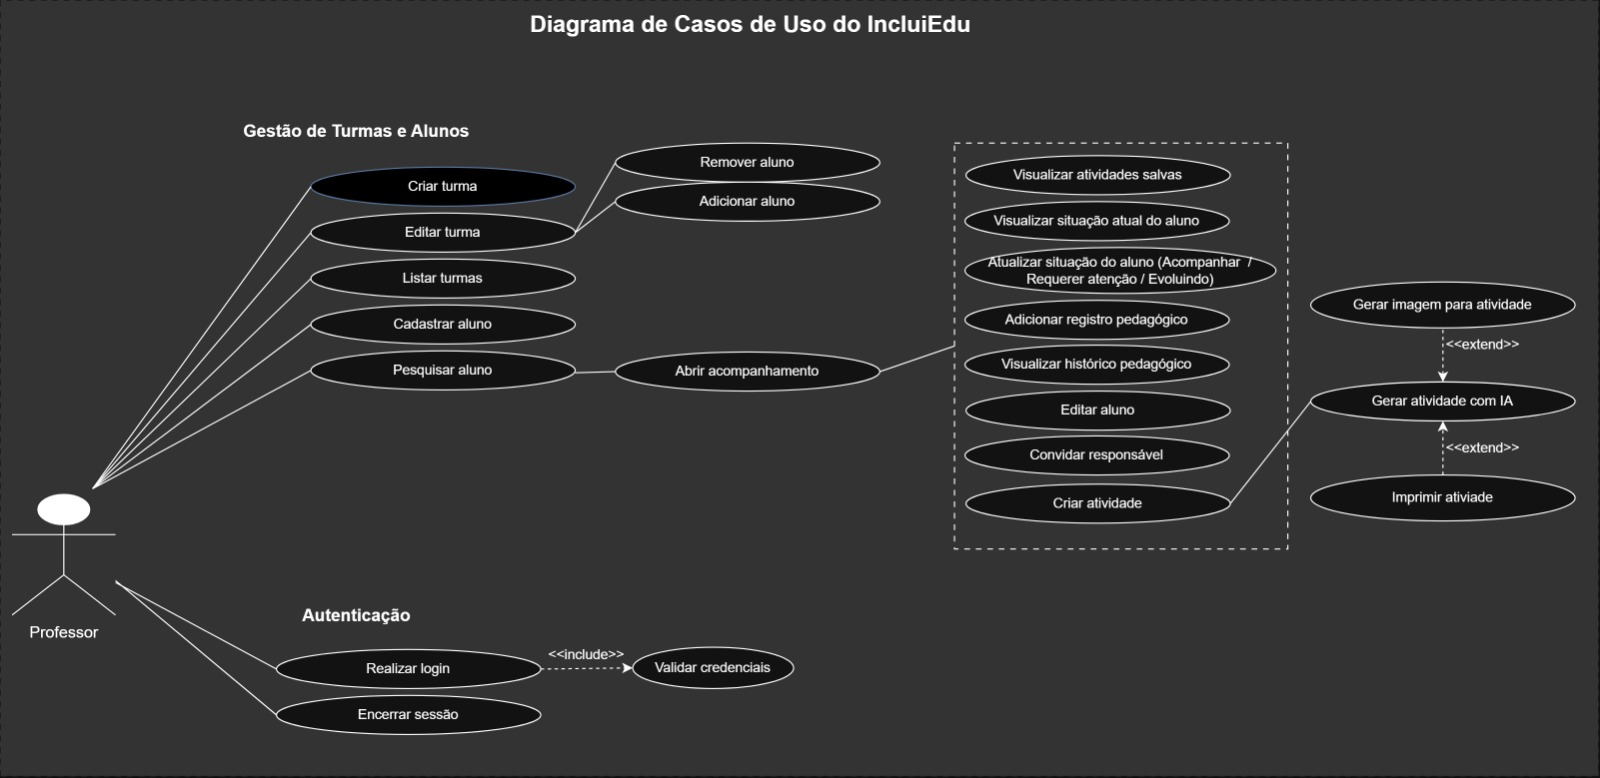
\includegraphics[width=0.9\textwidth]{04-figuras/casos_de_uso.jpeg}
    \fonte{Elaborado pelos autores (2026).}
\end{figure}

\subsection{DIAGRAMA DE CLASSES}
O diagrama de classes representa as principais entidades do sistema e seus relacionamentos. O professor está associado às turmas, que possuem alunos cadastrados. Cada aluno pode apresentar registros pedagógicos e atividades, permitindo a organização e a consulta das informações utilizadas no acompanhamento individual, conforme a Figura~\ref{fig:diagrama-classes}.

\begin{figure}[H]
    \centering
    \caption{Diagrama de Classes - IncluiEdu}
    \label{fig:diagrama-classes}
    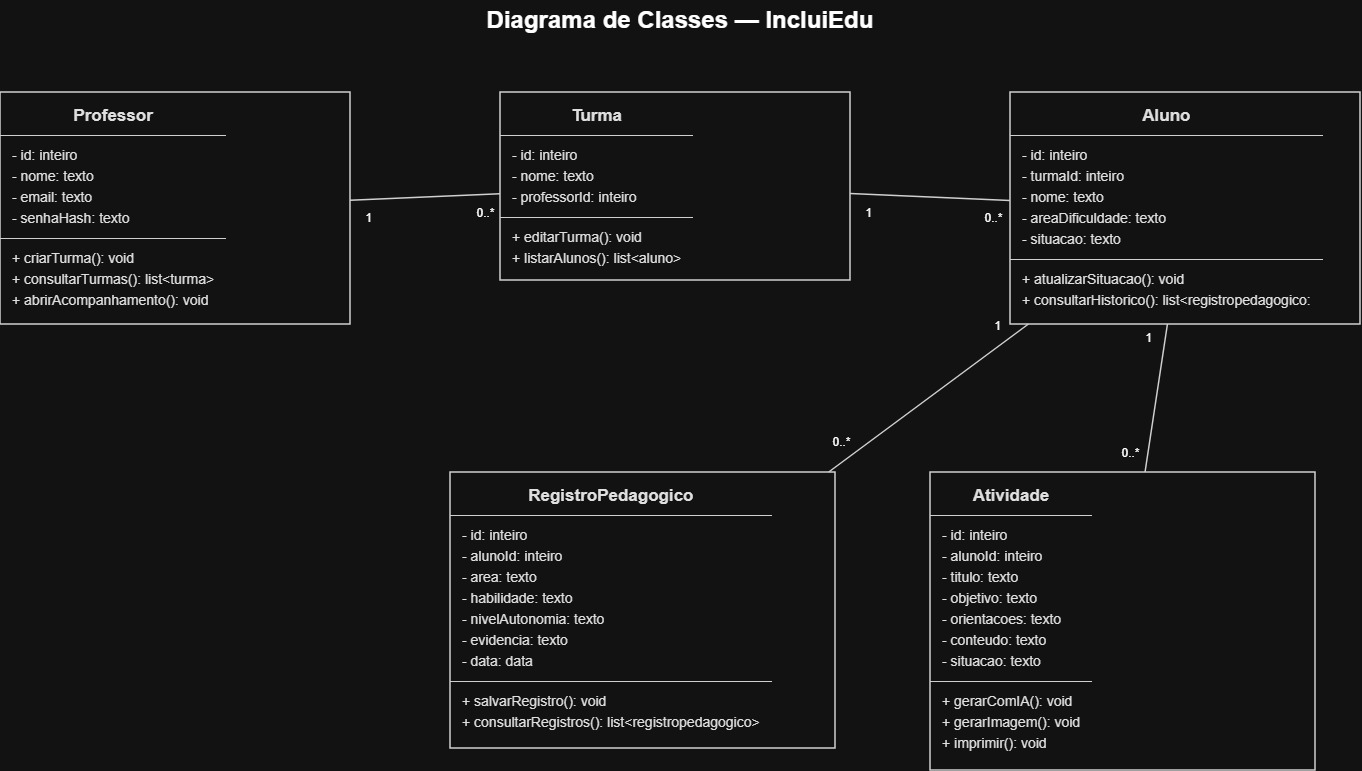
\includegraphics[width=0.9\textwidth]{04-figuras/diagrama_classes.jpeg}
    \fonte{Elaborado pelos autores (2026).}
\end{figure}

\subsection{MODELAGEM E IMPLEMENTAÇÃO DO BANCO DE DADOS}

A etapa local utilizou SQLite. Na versão atual, o Cloudflare D1 armazena dados em estrutura relacional \cite{cloudflare2026d1}. O modelo descrito compreende as entidades \texttt{users}, \texttt{classes}, \texttt{students}, \texttt{observations} e \texttt{activities}, relacionadas por chaves primárias e estrangeiras.

Um professor pode possuir diversas turmas; uma turma, diversos alunos; e cada aluno pode reunir observações e atividades ao longo do acompanhamento.

A estrutura do D1 é criada por migrações SQL, que documentam as tabelas e seus relacionamentos. As operações do backend utilizam instruções preparadas com parâmetros vinculados pelo método \texttt{.bind()}, evitando a concatenação direta dos valores recebidos em comandos SQL. O sistema verifica a vinculação dos registros ao professor autenticado antes de consultas ou alterações protegidas.

\begin{figure}[H]
    \centering
    \caption{Modelo do Banco de Dados - IncluiEdu}
    \label{fig:modelo-relacional}
    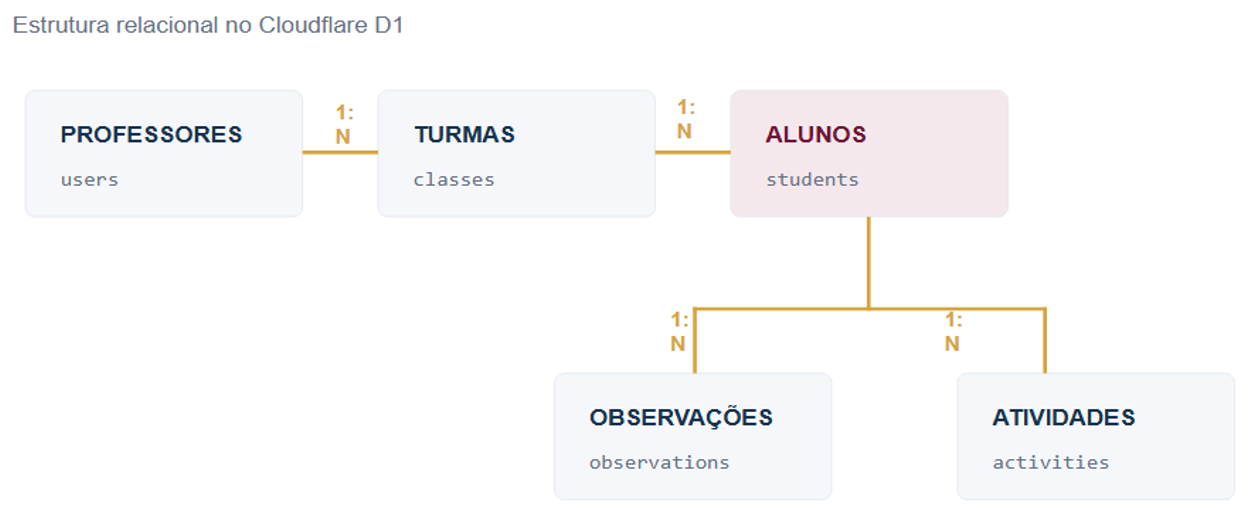
\includegraphics[width=0.9\textwidth]{04-figuras/modelo-relacional.png}
    \fonte{Elaborado pelos autores (2026).}
\end{figure}

\section{IMPLEMENTAÇÃO DO SISTEMA}

Na versão atual do IncluiEdu, a interface web apresenta as telas de cadastro, consulta e acompanhamento dos alunos. As ações realizadas pelo professor são enviadas à API por meio de requisições \texttt{fetch}, utilizando dados em formato JSON. O Cloudflare Worker recebe essas requisições, verifica a sessão e as permissões do usuário e realiza as operações necessárias no banco de dados D1. Em seguida, a resposta é enviada à interface, permitindo a atualização das informações apresentadas.

A autenticação utiliza derivação de senhas com PBKDF2, salt e SHA-256, evitando o armazenamento das senhas em texto simples. Após o login, o sistema cria uma sessão identificada por um cookie configurado com os atributos \texttt{HttpOnly}, \texttt{Secure} e \texttt{SameSite=Strict}. O backend também verifica se os registros acessados pertencem ao professor autenticado antes de permitir consultas ou alterações.

No acompanhamento pedagógico, cada registro reúne informações sobre o aluno, a área acompanhada, a habilidade observada, o nível de autonomia e as evidências registradas pelo professor. Esses dados são preservados no histórico pedagógico, permitindo acompanhar as observações realizadas ao longo do tempo. A situação do aluno também pode ser atualizada entre as opções \textit{Acompanhar}, \textit{Requer atenção} e \textit{Evoluindo}.

\section{TESTES E VALIDAÇÃO}

A verificação das funcionalidades do IncluiEdu foi realizada manualmente, por meio da interação com a aplicação. Os cenários de teste abrangem autenticação, organização de turmas, cadastro e consulta de alunos, observações pedagógicas, atualização da situação do aluno, geração de atividades e controle de acesso. Os procedimentos estão relacionados aos requisitos funcionais do sistema, conforme o Quadro~\ref{qua:testes}.

\begin{quadro}[htb]
\centering
\caption{Cenários de teste e resultados observados}
\label{qua:testes}
\small
\begin{tabular}{|p{2.5cm}|p{6cm}|p{5.5cm}|}
\hline
\textbf{Cenário} & \textbf{Procedimento realizado} & \textbf{Resultado} \\
\hline
Autenticação & Realização de login com credenciais válidas e inválidas. & O sistema permitiu o acesso com credenciais válidas e impediu a entrada com dados incorretos. \\
\hline
Turmas e alunos & Cadastro de turma e aluno, seleção de turma e pesquisa de aluno pelo nome. & As informações cadastradas foram exibidas corretamente, permitindo selecionar turmas e localizar alunos. \\
\hline
Acompanhamento & Abertura do acompanhamento individual de um aluno. & O sistema apresentou as informações do aluno, incluindo sua situação atual, registros pedagógicos e atividades salvas. \\
\hline
Registro pedagógico & Preenchimento dos campos de área, habilidade, nível de autonomia e evidência observada, seguido do salvamento. & O registro foi armazenado e disponibilizado para consulta no histórico pedagógico do aluno. \\
\hline
Situação do aluno & Alteração da situação entre \textit{Acompanhar}, \textit{Requer atenção} e \textit{Evoluindo}. & A situação foi atualizada e apresentada no perfil do aluno e no painel de acompanhamento. \\
\hline
Inteligência Artificial & Solicitação de uma atividade pedagógica personalizada por meio da IA. & O sistema apresentou uma atividade contendo título, objetivo, orientações e conteúdo pedagógico, identificada como rascunho para revisão. \\
\hline
Geração de imagem & Utilização da opção de gerar imagem para uma atividade produzida pela IA. & O sistema gerou uma imagem relacionada à atividade pedagógica solicitada, disponibilizando o resultado para utilização pelo professor. \\
\hline
Encerramento de sessão & Utilização da opção \textit{Sair} após autenticação. & A sessão foi encerrada, retornando o usuário à área de autenticação. \\
\hline
Controle de acesso & Tentativa de consultar registros de outro professor utilizando uma conta diferente. & O sistema impediu o acesso aos registros vinculados ao outro professor. \\
\hline
\end{tabular}
\fonte{Elaborado pelos autores (2026).}
\end{quadro}

Os testes manuais foram direcionados à observação do comportamento da versão atual da plataforma. A avaliação considerou os fluxos de utilização do professor e a comunicação entre interface, backend e serviços integrados.

\section{IMPLANTAÇÃO E REPRODUTIBILIDADE}

O IncluiEdu encontra-se publicado na plataforma Cloudflare, permitindo o acesso à aplicação por meio de um navegador web. A configuração do ambiente é organizada no arquivo \texttt{wrangler.jsonc}, que estabelece os vínculos necessários para o funcionamento dos serviços utilizados.

O código-fonte do projeto é mantido em um repositório no GitHub. Para reproduzir a aplicação em outro ambiente, é necessário obter os arquivos do projeto, configurar os serviços da Cloudflare, preparar o banco de dados D1 e realizar a publicação da aplicação.
        %
% Documento: Estrutura
%

\chapter{RESULTADOS}

A estrutura de acordo com a NBR-14724, compreende três elementos: pré-textuais, tex-tuais e pós-textuais.

\begin{figure}[H]
	\vspace*{0,2cm}
    \centering
    \caption{Ilustração da estrutura}
    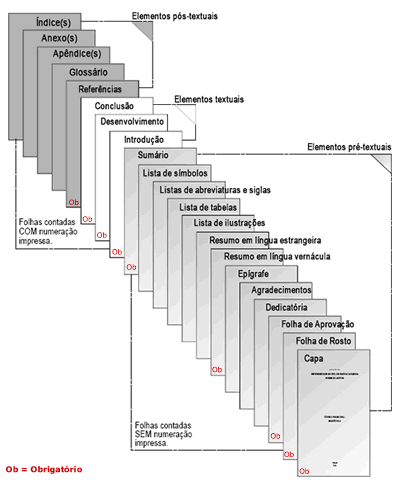
\includegraphics[width=0.6\textwidth]{./04-figuras/abnt}
    \label{fig:ilustfig2}
\end{figure}
\vspace*{-0,9cm}
{\raggedright \fonte{Disponível em: <https://www.intelligentsia.zip.net/estruturamonografia>. Acesso em: 15 ago. 2014.}}\\


\chapter{CONCLUSÃO}
Os Trabalhos de Conclusão de Curso (TCC) são documentos que
representam o resultado de estudo, devendo expressar conhecimento do assunto escolhido. Deve ser emanado da disciplina, módulo, estudo independente, curso, programa e outros ministrados. Deve ser feito sob a coordenação de um orientador.
A norma que determina os trabalhos com esse fim é a NBR 14724. Nesse documento será usada documentação o ABNTEX disponivel no site
\chapter{AGRADECIMENTOS}




    
        \include{./02-elementos-textuais/ambientes}  	
        %
% Documento: Citações
%

\section{Citações (ABNT NBR 10520)}

Esta seção apresenta exemplos práticos de citação conforme a ABNT NBR 10520.

\subsection{Citação direta curta (até 3 linhas)}
Deve permanecer no corpo do parágrafo, entre aspas duplas, com indicação de autor, ano e página:
\begin{flushleft}
\textit{Ex.:} De acordo com \citeonline[p.~249]{marshall1980}, ``não se pode discutir se o valor e os preços são governados pela utilidade ou pelo custo de produção''.
\end{flushleft}

Outras variações úteis:
\begin{itemize}
  \item Autor no texto + ano entre parênteses: \citeauthor{marshall1980} (\citeyear{marshall1980}) afirma que ``\ldots'' \cite[p.~249]{marshall1980}.
  \item Apenas referência entre parênteses: ``\ldots'' \cite[p.~249]{marshall1980}.
\end{itemize}

\subsection{Citação direta longa (mais de 3 linhas)}
Deve ir em bloco destacado, com recuo de 4\,cm da margem esquerda, fonte menor e sem aspas. 
No \texttt{abntex2}, use o ambiente \texttt{citacao}, que já aplica o padrão:
\begin{citacao}
Da mesma forma que não se pode afirmar se é a lâmina inferior ou superior de uma tesoura que corta uma folha de papel, também não se pode discutir se o valor e os preços são governados pela utilidade ou pelo custo de produção. (MARSHALL, 1980, p.~249)
\end{citacao}

\subsection{Citação indireta (paráfrase)}
Reproduz a ideia do autor com suas palavras. Página é opcional; recomenda-se quando ajuda o leitor.
\begin{flushleft}
\textit{Ex.:} A produção acadêmica sobre varejo no Brasil é desproporcional à relevância do segmento na economia \cite{angelo1993}.
\end{flushleft}
Variações:
\begin{itemize}
  \item \citeauthor{angelo1993} (\citeyear{angelo1993}) argumentam que \ldots
  \item Conforme apontado na literatura \cite{tanenbaum1995sistemas,de2017sistema}, \ldots
\end{itemize}

\subsection{Citação de citação (apud)}
Use somente quando o original não puder ser consultado. Indique o autor original, seguido de ``apud'' e do autor efetivamente consultado, com página.
\begin{flushleft}
\textit{Ex. no corpo do texto:} Enguita (apud \citeauthor{silva1991}, \citeyear{silva1991}, p.~21) chegou às mesmas conclusões.
\end{flushleft}

Também é possível registrar em nota de rodapé a fonte consultada:
\begin{flushleft}
\textit{Ex. com nota:} Enguita\footnote{Informação citada por \citeauthor{silva1991} (\citeyear{silva1991}, p.~21).} chegou às mesmas conclusões.
\end{flushleft}

\subsection{Comandos úteis (abntex2cite)}
\begin{itemize}
  \item \verb|\cite{chave}| → (AUTOR, ano)
  \item \verb|\citeonline{chave}| → AUTOR (ano)
  \item \verb|\citeauthor{chave}| → AUTOR
  \item \verb|\citeyear{chave}| → ano
  \item \verb|\cite[p.~10]{chave}| → (AUTOR, ano, p.~10)
\end{itemize}

\subsection{Observações finais}
\begin{itemize}
  \item Para siglas: escreva por extenso na primeira ocorrência, seguidas da sigla: Associação Brasileira do Trabalhador (ABT).
  \item As referências completas devem aparecer na lista de referências ao final do trabalho.
\end{itemize}

  	
    
\end{OnehalfSpacing}

    % Elementos pós-textuais
    \postextual
    %
% Documento: Referências Bibliográficas
%

\bibliography{referencias}    % Geração automática das referências por meio do arquivo 'referencias.bib'
       

\end{document}
\documentclass[oneside]{estilo}

% Importações de pacotes
\usepackage[alf, abnt-emphasize=bf, recuo=0cm, abnt-etal-cite=2, abnt-etal-list=0]{abntex2cite}  % Citações padrão ABNT
\usepackage[utf8]{inputenc}                         % Acentuação direta
\usepackage[T1]{fontenc}                            % Codificação da fonte em 8 bits
\usepackage{graphicx}                               % Inserir figuras
\usepackage{amsfonts, amssymb, amsmath}             % Fonte e símbolos matemáticos
\usepackage{booktabs}                               % Comandos para tabelas
\usepackage{verbatim}                               % Texto é interpretado como escrito no documento
\usepackage{multirow, array}                        % Múltiplas linhas e colunas em tabelas
\usepackage{indentfirst}                            % Endenta o primeiro parágrafo de cada seção.
\usepackage{microtype}                              % Para melhorias de justificação
\usepackage[algoruled, portuguese]{algorithm2e}     % Escrever algoritmos
\usepackage{float}                                  % Utilizado para criação de floats
%\usepackage{times}                                 % Usa a fonte Times

\usepackage{color}
\usepackage{chronosys}
\usepackage{pdflscape}
\usepackage{tabu}
\usepackage{makecell}
\usepackage{nameref}
\usepackage{listings}
\usepackage{enumitem}
\usepackage{chngcntr}
\usepackage{colortbl}
\usepackage[htt]{hyphenat}
\usepackage{mdframed}

\mdfsetup{skipabove=1.5\topskip,skipbelow=0.5\topskip}
\mdfdefinestyle{pp}{%
	linecolor=black,
	outerlinewidth=.5pt,
	roundcorner=5pt,
	innertopmargin=8pt,
	innerbottommargin=0.5\baselineskip,
	usetwoside=false
}

%\usepackage{minitoc}
%\dominitoc% Initialization
\newcommand{\enumerateletter}[2]{\textbf{#1\textsubscript{#2}}}

% Inclui o preâmbulo do documento
%
% Documento: Preâmbulo + Capa
%

% -------------------------------
% Pacotes necessários
% -------------------------------
\usepackage{lmodern}     % Fonte Latin Modern
\usepackage{listings}    % Ambientes de código
\usepackage{tocloft}     % Personalização das listas
\usepackage{chngcntr}    % Necessário para \counterwithin

% -------------------------------
% Configuração de listagens
% -------------------------------
\renewcommand{\lstlistingname}{Código}

\counterwithin{figure}{chapter}
\counterwithin{table}{chapter}

% Criação da "Lista de Códigos" conforme ABNT
\begingroup\makeatletter
\let\newcounter\@gobble
\let\setcounter\@gobbletwo
\globaldefs\@ne
\let\c@loldepth\@ne
\newlistof{listings}{lol}{\lstlistlistingname}
\newlistentry{lstlisting}{lol}{0}
\endgroup

\renewcommand{\cftlstlistingaftersnum}{\hfill--\hfill}

\let\oldlstlistoflistings\lstlistoflistings
\renewcommand{\lstlistoflistings}{%
  \begingroup%
  \let\oldnumberline\numberline%
  \renewcommand{\numberline}{\lstlistingname\space\oldnumberline}%
  \oldlstlistoflistings%
  \endgroup}

% Estilo para códigos
\lstdefinestyle{master-thesis}{
  basicstyle=\ttfamily\small,
  numbers=left,
  numberstyle=\tiny,
  frame=tb,
  columns=fullflexible,
  showstringspaces=false,
  captionpos=b,
  breaklines=true,
  tabsize=2
}
\lstset{style=master-thesis}

% -------------------------------
% ==== DADOS DA CAPA (ÚNICO LUGAR PARA EDITAR) ====


\instituicao{UNIFIO - CENTRO UNIVERSITÁRIO DE OURINHOS}
\departamento{CURSO: ENGENHARIA DE SOFTWARE}
\titulotb{SISTEMA DE APOIO A PROFESSORES DO ENSINO FUNDAMENTAL PARA CRIAÇÃO DE ATIVIDADES ADAPTADAS A CRIANÇAS NEURODIVERGENTES}

\nomeautor{%
  \textbf{EDSON CARLOS VICENTIM JUNIOR}\\
  \textbf{MIGUEL ANGELO BURATI MORALEZ}\\
  \textbf{PEDRO HENRIQUE SILVÉRIO DA FONSECA}\\
  \textbf{VICTOR AUGUSTO MOREIRA BARBOSA}%
}

\localapresentacao{Ourinhos -- São Paulo}
\anoapresentacao{2026}


\usepackage[a4paper, top=3.0cm, bottom=2.0cm, left=3.0cm, right=2.0cm]{geometry} %teste margem

\newcommand{\blue}[1]{\textcolor{blue}{#1}} % proposed
\newcommand{\red}[1]{\textcolor{red}{#1}} % to be removed
\newcommand{\green}[1]{\textcolor{green}{#1}} % to be discussed?
\newcommand{\magenta}[1]{\textcolor{magenta}{#1}} % warning - requires attention

\settocdepth{subsection}

% Define as cores dos links e informações do PDF
\makeatletter
\hypersetup{
    portuguese,
    colorlinks,
    linkcolor=blue,
    citecolor=blue,
    filecolor=black,
    urlcolor=black,
    breaklinks=true,
    pdftitle={\imprimirtitulotb},
    pdfauthor={\imprimirnomeautor}
}
\makeatother

% Redefinição de labels
\renewcommand{\algorithmautorefname}{Algoritmo}
\def\equationautorefname~#1\null{Equa\c c\~ao~(#1)\null}

% Cria o índice remissivo
\makeindex

% Início do documento
\begin{document}

    % Retira espaço extra obsoleto entre as frases.
    \frenchspacing

    % Elementos pré-textuais
    \pretextual
    \include{01-elementos-pre-textuais/dados}       % único lugar onde você edita capa
    %
% Documento: Capa
%

\makeatletter
\begin{capa}
	\thispagestyle{empty}%limpa estilo da pagina
	\setlength{\baselineskip}{0.72\baselineskip}
    \begin{center} %Alinhamento centralizado
	

    \textbf{\expandafter\uppercase\expandafter{\imprimirinstituicao}}\\
    \textbf{\expandafter\uppercase\expandafter{\imprimirdepartamento}}\\
    %\textbf{\expandafter\uppercase\expandafter{\imprimirprograma}}\\
	\vspace*{5cm}%Espaçamento entre linhas
	\large\textbf{\expandafter\uppercase\expandafter{\imprimirtitulotb}}\\
	\vspace*{6cm}%Espaçamento entre linhas	
	\small\textbf{\expandafter\uppercase\expandafter{\imprimirnomeautor}}\\
	\vspace*{6.5cm}%%Espaçamento entre linhas
	\large\textbf{\expandafter\expandafter{\imprimirlocalapresentacao, \imprimirdataapresentacao}}
	%\small\textbf{\expandafter\uppercase\expandafter{\imprimirdata}}\\
		
		
		
	\end{center} %Alinhamento centralizado
\end{capa}
\makeatother

	

        % imprime a capa
    \include{01-elementos-pre-textuais/resumoPt}    % Resumo na língua vernácula
    %
% Documento: Resumo (Inglês)
\begin{RESUMO}
\thispagestyle{empty}
	aqui é o resumo
		\noindent Etc.

		\vspace*{0.5cm}\noindent\textbf{Palavras-chave}: Etc etc.
		

\end{RESUMO}

\begin{ABSTRACT}
	
		\noindent Etc.

		\vspace*{0.5cm}\noindent\textbf{Keywords}: Etc. Etc. Etc.
		
\end{ABSTRACT}
    % Resumo em língua estrangeira
    %
% Documento: Lista de figuras
%

\pdfbookmark[0]{\listfigurename}{lof}
\listoffigures*
\cleardoublepage

% Lista de figuras
   % \include{01-elementos-pre-textuais/listaTabelas}

    \sumario
\begin{OnehalfSpacing}

    % Elementos textuais
    \textual
        %
% Documento: Introdução
\setcounter{page}{6}
\chapter{INTRODUÇÃO}\label{chap:introducao}


Os Trabalhos de Conclusão de Curso (TCC) são documentos que
representam o resultado de estudo, devendo expressar conhecimento do assunto escolhido. Deve ser emanado da disciplina, módulo, estudo independente, curso, programa e outros ministrados. Deve ser feito sob a coordenação de um orientador.
A norma que determina os trabalhos com esse fim é a NBR 14724. Nesse documento será usada documentação o ABNTEX disponivel no site \href{https://code.google.com/p/abntex2/}{https://code.google.com/p/abntex2/} .

\section{PROBLEMA}

\section{OBJETIVOS}
\subsection{OBJETIVO GERAL}
\subsection{OBJETIVOS ESPECÍFICOS}
\section{JUSTIFICATIVA}




        %
% Documento: Tecnicas de referencia
%

\chapter{FUNDAMENTAÇÃO TEÓRICA}

\section{EDUCAÇÃO INCLUSIVA E DEFICIÊNCIA INTELECTUAL NO BRASIL}

A legislação brasileira garante o direito à educação inclusiva para alunos com deficiência intelectual (DI) \cite{brasil2015lbi}, mas a realidade da escola pública revela uma lacuna significativa entre o que a lei prevê e o que o professor consegue executar \cite{souza2025acessibilidade}. O educador não possui formação específica nem tempo hábil para dominar os diferentes perfis neurodivergentes presentes em uma mesma turma \cite{irm2026panorama}, resultando em uma inclusão que frequentemente se limita à presença física, sem garantir aprendizagem efetiva \cite{oliveira2025escolas}. É nessa lacuna que o sistema proposto se insere.

\subsection{BASE LEGAL}

A educação inclusiva no Brasil está fundamentada principalmente na Lei nº 13.146/2015 \cite{brasil2015lbi}, que assegura o direito das pessoas com deficiência à educação preferencialmente na rede regular de ensino. Complementarmente, o Decreto nº 10.502/2020 \cite{brasil2020pnee} instituiu diretrizes para o Atendimento Educacional Especializado (AEE), determinando que os profissionais da educação recebam formação orientada à atuação efetiva em espaços comuns ou especializados. Importante registrar que esse decreto foi revogado em 1º de janeiro de 2023 pelo Decreto nº 11.370 \cite{brasil2023revogacao}, o que evidencia a instabilidade das políticas de educação especial no país e reforça a necessidade de soluções que não dependam exclusivamente de marcos legais específicos.

\subsection{CRESCIMENTO DAS MATRÍCULAS}

Dados do Censo Escolar evidenciam a magnitude do desafio. Em 2025, havia aproximadamente 2,4 milhões de estudantes com alguma deficiência matriculados na educação básica brasileira, um crescimento de 153\% em relação a 2016 \cite{inep2025censo}. Desse total, a deficiência intelectual representa cerca de 43\% dos casos, sendo a categoria mais numerosa dentro da educação especial \cite{inep2025censo}. Esses números indicam que o 5 professor da escola pública muito provavelmente encontrará mais de um aluno com DI na mesma turma, cada um com características, ritmos e necessidades de apoio distintos.

\subsection{A LACUNA ENTRE A LEI E A PRÁTICA}

Pesquisas recentes na área educacional brasileira apontam de forma consistente
que a inclusão de alunos com DI ainda é um processo em construção. Um estudo qualitativo
realizado em escolas de Salvador-BA, com professores do 2º ao 4º ano e profissionais do
AEE, identificou que a falta de formação docente e o suporte institucional insuficiente
estão entre os principais obstáculos à efetivação da inclusão \cite{souza2025acessibilidade}.
O mesmo estudo, no entanto, reconhece que práticas inclusivas eficazes existem, como
adaptações curriculares, uso de objetos concretos e estratégias centradas no ritmo de cada
estudante, mas dependem de condições que nem sempre estão disponíveis.
Outra investigação, publicada na Revista Foco (\citeyear{oliveira2025escolas}), reforça esse panorama
ao elencar os desafios enfrentados pelas escolas regulares: falta de recursos pedagógicos
adaptados, ausência de formação continuada voltada para a inclusão e barreiras atitudinais
\cite{oliveira2025escolas}. O estudo destaca que, para que a inclusão de alunos com DI
seja efetiva, não basta garantir o acesso à escola; é necessário assegurar participação plena
e aprendizagem significativa.

\subsection{A DIFICULDADE ESPECÍFICA DO PROFESSOR}

A literatura aponta que o professor do ensino regular, em sua maioria, não recebeu formação inicial adequada para trabalhar com alunos com DI. Um estudo realizado no Piauí com professores dos anos iniciais do Ensino Fundamental revelou que, embora os docentes demonstrem conhecimento teórico sobre Educação Especial, eles enfrentam dificuldades concretas na sala de aula, como estrutura física inadequada e escassez de recursos didático-pedagógicos \cite{oliveira2025escolas}. A pesquisa também identificou que os professores se esforçam para propor atividades diferenciadas, mas o fazem sem o suporte necessário. Um ponto crítico emerge dessa literatura \cite{oliveira2025escolas}: o professor precisaria estudar cada perfil neurodivergente separadamente para conseguir planejar atividades minimamente adequadas. Considerando que uma turma pode ter alunos neurodivergentes associados a diferentes condições (dificuldades cognitivas, de linguagem, de atenção, entre outras), essa tarefa torna-se inviável dentro da carga horária docente. O resultado é que a inclusão, muitas vezes, acaba se reduzindo à socialização: a criança permanece na sala, mas não necessariamente acessa o conhecimento.

\section{DIFICULDADES ESTRUTURAIS E FINANCEIRAS DA ESCOLA PÚBLICA NO ENSINO DE ALUNOS COM DI}

O professor da escola pública enfrenta uma combinação de dificuldades que vão muito além da falta de formação inicial \cite{irm2026panorama}. A ausência de incentivo financeiro para capacitação, a precariedade de recursos materiais, a insuficiência de profissionais especializados e a sobrecarga de trabalho tornam praticamente impossível o ensino adequado de alunos com deficiência intelectual (DI) \cite{cunha2025recursos, lievore2025financiamento}. Essas barreiras são estruturais e afetam diretamente a qualidade da inclusão.

\subsection{FALTA DE FORMAÇÃO CONTINUADA E AUSÊNCIA DE ICENTIVO FINANCEIRO}Os dados do Censo Escolar 2025 revelam uma realidade preocupante: apenas
11,3\% dos gestores escolares possuíam formação continuada em educação inclusiva em
2025, um número que, embora tenha crescido em relação a 2019 (5,8\%), ainda está muito
aquém do necessário \cite{irm2026panorama}. Mais crítico ainda é o dado sobre os professores
regentes: em 2024, apenas 6,4\% dos docentes tinham formação continuada em Educação
Especial, totalizando 151 mil professores com essa formação em um universo de 2,4 milhões
de docentes no país \cite{irm2026panorama}.
Essa lacuna não é acidental. A ausência de incentivo financeiro é um dos principais
fatores que impedem o professor da rede pública de buscar capacitação. Cursos de especialização em Educação Especial ou Psicopedagogia são pagos e, para um professor com
jornada dupla ou tripla, representam um custo financeiro e de tempo inviável. Além disso,
as escolas frequentemente não oferecem tempo remunerado para estudo nem parcerias
estruturadas com universidades para formação continuada \cite{educacaointegral2026}.
A pesquisa acadêmica confirma esse cenário: dados de um estudo com professores
apontam que a escassez de recursos foi apontada por 60\% dos participantes como um
problema, e a ausência de recursos que prejudicam o processo de ensino-aprendizagem foi
confirmada por 86,6\% (somando concordância e concordância forte) \cite{cunha2025recursos}. A
falta de investimento público necessário para viabilizar práticas inclusivas é uma barreira
estrutural que se agrava em contextos de restrição orçamentária.

\subsection{PRECARIEDADE DE RECURSOS MATERIAIS E INFRAESTRUTRA}

Além da formação, a escola pública carece de recursos materiais básicos para a
inclusão. Mais de 20\% das escolas brasileiras não possuem nenhum item de acessibilidade
física registrado \cite{irm2026panorama}. Entre as que possuem, os recursos mais comuns
são rampas (57,6\%), banheiro adaptado (54,8\%), vão livre (43,4\%) e corrimão (34,2\%)
\cite{irm2026panorama}.
7
Quando se trata de recursos pedagógicos adaptados, materiais concretos, jogos
educativos e tecnologia assistiva, a situação é ainda mais crítica. Um estudo sobre a
implementação de políticas inclusivas em escolas públicas revelou que 46,6\% dos professores
concordaram e 40\% concordaram fortemente que a ausência de recursos prejudica o processo
de ensino-aprendizagem, enquanto 60\% \cite{cunha2025recursos}. Isso demonstra que, mesmo
quando existem alguns recursos, eles são insuficientes para atender à demanda real.
A demora na disponibilização de recursos também foi apontada como barreira:
80\% dos participantes (somando concordância e concordância forte) relataram lentidão
nos processos administrativos para aquisição de materiais \cite{cunha2025recursos}. Isso evidencia
entraves burocráticos que impactam diretamente o cotidiano da sala de aula.


\subsection{FALTA DE PROFISSIONAIS ESPECIALIZADOS E SOBRECARGA DOCENTE}

Outro problema estrutural é a insuficiência de equipes multiprofissionais nas
escolas públicas. Um relato de escuta pública em Amaralina (GO) destacou a necessidade
urgente de ampliar a equipe multiprofissional, com psicólogos, terapeutas ocupacionais e
fonoaudiólogos, para atender adequadamente alunos neuroatípicos \cite{mpeduc2025}.
No Distrito Federal, a situação chegou a um ponto crítico: nos 13 Centros de
Ensino Especial, salas com até quatro professores atendiam apenas três alunos, gerando
superlotação, não pelo número absoluto, mas pela demanda por acompanhamento individualizado que supera a capacidade das equipes \cite{forum2026df}. Uma professora relatou ter
sido agredida por um aluno com TEA que não recebia o suporte necessário, evidenciando
o impacto da falta de profissionais na segurança e no bem-estar de todos \cite{forum2026df}.
Esse cenário se agrava com a sobrecarga do professor regente, que precisa dar
conta de uma turma diversa, com alunos de diferentes perfis neurodivergentes, sem o
apoio de especialistas. A consequência é que a inclusão, muitas vezes, acaba se reduzindo
à socialização: o aluno permanece na sala, mas não acessa o conhecimento de forma
significativa.

\subsection{A DEPÊNDENCIA DE RECURSOS EXTERNOS E A LÓGICA DO DESINVESTIMENTO}

A pesquisa acadêmica aponta uma questão estrutural mais profunda: a desarmonia
entre as políticas públicas formuladas e a efetiva reserva orçamentária destinada ao seu
cumprimento \cite{lievore2025financiamento}. Embora o Brasil tenha uma legislação robusta
sobre inclusão \cite{brasil2015lbi, brasil2020pnee}, os avanços normativos não foram acompanhados por
mecanismos financeiros compatíveis com as exigências pedagógicas, estruturais e humanas
da Educação Especial \cite{lievore2025financiamento}.
8
Um estudo sobre a Meta 4 do Plano Nacional de Educação (2014–2024) confirma
esse diagnóstico: houve avanços normativos e aumento de recursos via Fundeb, mas não
houve ampliação da cobertura do Atendimento Educacional Especializado nas
redes públicas de ensino \cite{franca2025financiamento}. Os dados mostram que o percentual
de matrículas na Educação Básica de alunos de 4 a 17 anos com deficiência, TGD, altas
habilidades ou superdotação que recebem AEE apresentou decréscimo no período,
de 50\% em 2014 para 47\% em 2023 \cite{franca2025financiamento}. Além disso, os
valores destinados à Educação Especial via PDDE (Programa Dinheiro Direto na Escola)
apresentaram decréscimos significativos no período de 2019 a 2022, que podem estar
relacionados aos efeitos pandêmicos, mas também à política de austeridade fiscal imposta
pela Emenda Constitucional nº 95/2016 \cite{franca2025financiamento}.
A lógica do desinvestimento na Educação Especial é agravada quando a educação
passa a ser concebida sob uma ótica de retorno econômico. Áreas de menor “atratividade
mercadológica”, como a Educação Especial, tendem a sofrer recorrentes desinvestimentos
estruturais e operacionais \cite{lievore2025financiamento}. Isso significa que, sem pressão política
e social, a tendência é que os recursos para a inclusão de alunos com DI permaneçam
insuficientes.

\section{INTELIGÊNCIA ARTIFICIAL GENERATIVA COMO FERRAMENTA
DE APOIO AO PROFESSOR}

A terceira subseção apresenta a IA generativa como solução tecnológica viável para o problema estrutural exposto na subseção anterior. A ferramenta se posiciona como apoio à decisão docente, e não como substituta do professor.

\subsection{IA GENERATIVA E O PROBLEMA DA ESCOLA PÚBLICA}

A IA generativa (GenAI) refere-se a sistemas baseados em grandes modelos de linguagem (LLMs) capazes de produzir texto, imagens e outros conteúdos a partir de comandos em linguagem natural \cite{engaja2026}. Diferentemente de tecnologias assistivas tradicionais, a GenAI pode gerar conteúdo novo e contextualizado, reescrever textos em diferentes níveis de complexidade, criar atividades adaptadas e sugerir estratégias pedagógicas sob demanda.

No contexto da escola pública brasileira, essa capacidade é particularmente relevante. Como demonstrado na subseção anterior, o professor enfrenta falta de formação continuada, ausência de incentivo financeiro, precariedade de recursos e sobrecarga de trabalho \cite{irm2026panorama, cunha2025recursos}. A IA generativa pode atuar como ferramenta de apoio para reduzir parte dessa carga, oferecendo um ponto de partida para a adaptação de atividades.

\subsection{O PROFESSOR NO CONTROLE: ATIVIDADE COMO RASCUNHO}

A IA generativa não substitui o professor. Toda atividade produzida é armazenada com status de rascunho, o que significa que:

\begin{itemize}
    \item A atividade não é publicada automaticamente para o aluno;
    \item O professor precisa revisar, corrigir e adaptar antes de utilizá-la;
    \item A decisão pedagógica final permanece humana.
\end{itemize}

Esse mecanismo está alinhado à literatura sobre IA na educação inclusiva \cite{engaja2026}, que alerta para riscos como viés algorítmico, alucinações e padronização excessiva. A revisão humana obrigatória é uma barreira de segurança pedagógica e ética.

\section{TRABALHOS CORRELATOS}
A EDUNIA é uma plataforma de educação especial e inclusiva que utiliza IA para personalizar atividades pedagógicas. O professor ou responsável fornece informações sobre o estudante (anamnese, arquivo ou fotografia de atividade) e interesses da criança, e a plataforma gera uma atividade adaptada, disponível em PDF, alinhada à BNCC. A ferramenta contempla estudantes com TEA, TDAH e outras necessidades educacionais \cite{edunia2026}.

A Inklua é uma plataforma de gestão da Educação Especial e Inclusiva que centraliza informações dos estudantes e auxilia no planejamento, acompanhamento e documentação. Utiliza IA para auxiliar na criação de PAEE, PEI e atividades adaptadas, além de oferecer recursos para planos de aula, monitoramento da aprendizagem e avaliação de habilidades \cite{inklua2026}.

A Vínculoo é uma plataforma digital de educação especial e inclusiva que utiliza IA para apoiar professores no acompanhamento e planejamento pedagógico. Seu recurso \textit{Apoio Inteligente} analisa laudos, relatórios e observações para sugerir metas e estratégias pedagógicas, auxiliando na elaboração de PEI e PAEE e na adaptação de atividades. A plataforma enfatiza que a IA não substitui a decisão do professor, apresentando suas produções como sugestões editáveis \cite{vinculoo2026}.

No âmbito acadêmico, SALINA (\citeyear{salina2022lps}) apresenta uma abordagem de linhas de produto de software aplicada ao gerenciamento de atividades escolares, com instanciação direcionada a alunos com deficiência intelectual. Já NASCIMENTO; BATISTA; PEDERIVA (\citeyear{nascimento2024software}) abordam o desenvolvimento e a aplicação de um software educacional voltado para alfabetização e letramento de crianças com deficiência intelectual.

Esses trabalhos mostram que a busca por soluções tecnológicas para a educação inclusiva já é objeto de diferentes iniciativas, tanto no mercado quanto na academia. No entanto, a maioria das plataformas analisadas concentra-se em gestão, documentação, acompanhamento pedagógico ou adaptação de materiais de forma mais ampla, enquanto o presente trabalho se propõe a apoiar a criação de atividades adaptadas com foco em professores do ensino fundamental, considerando limitações do contexto escolar público e a necessidade de revisão humana no processo de geração de conteúdo. O Quadro 1 sintetiza a lacuna que este trabalho se propõe a preencher.

\begin{table}[h!]
\centering
\caption{Lacuna identificada em relação aos trabalhos correlatos}
\label{tab:lacuna}
\begin{tabular}{|p{3.5cm}|p{4cm}|p{5cm}|}
\hline
\textbf{Solução} & \textbf{Foco principal} & \textbf{Limitação em relação ao presente trabalho} \\
\hline
EDUNIA & Personalização de atividades com base em interesses e BNCC & Voltada ao professor ou responsável, sem foco explícito nas limitações da escola pública \\
\hline
Inkluo & Gestão e documentação da Educação Especial & Ênfase em gestão, não na criação de atividades adaptadas \\
\hline
Vínculoo & Acompanhamento pedagógico e elaboração de PEI/PAEE & Foco em planejamento e documentação, não na geração de atividades \\
\hline
SALINA (2022) & Linhas de produto de software para gestão de atividades & Abordagem acadêmica de gestão, não de geração de conteúdo adaptado \\
\hline
NASCIMENTO; BATISTA; PEDERIVA (2024) & Software educacional para alfabetização e letramento & Escopo restrito à alfabetização, sem apoio amplo à adaptação curricular \\
\hline
\textbf{Presente trabalho} & \textbf{Criação de atividades adaptadas para professores do ensino fundamental} & \textbf{Considera limitações do contexto escolar público e exige revisão humana obrigatória} \\
\hline
\end{tabular}
\end{table}
        %
% Documento: Disposições
%

\chapter{MATERIAIS E MÉTODOS}

\section{Materiais e ambiente de desenvolvimento}

O desenvolvimento do IncluiEdu envolveu duas configurações tecnológicas. Na etapa inicial, executada localmente, foram utilizados Python e Django para a aplicação, SQLite para armazenamento e Ollama para integração com inteligência artificial. Posteriormente, a versão atual passou a utilizar JavaScript e TypeScript, com backend em Cloudflare Workers, banco relacional Cloudflare D1 e geração de atividades por meio do Workers AI, com o modelo Gemma \cite{cloudflare2026workersai,cloudflare2026gemma,cloudflare2026d1}.

A interface web utiliza HTML, CSS e JavaScript para apresentar os recursos ao professor e comunicar-se com a API por requisições HTTP e dados em JSON. Na arquitetura atual, o arquivo \texttt{wrangler.jsonc} concentra a configuração do Worker, os vínculos com o banco de dados, o serviço de IA e os arquivos da interface. O código do projeto é mantido no GitHub.

A arquitetura atual utiliza serviços da Cloudflare para executar o backend, armazenar os registros e integrar a geração de atividades com inteligência artificial. O Cloudflare Workers processa as requisições da aplicação, o Cloudflare D1 mantém os dados relacionais e o Workers AI disponibiliza o modelo Gemma para a elaboração das propostas pedagógicas \cite{cloudflare2026workersai,cloudflare2026gemma,cloudflare2026d1}.

\section{Metodologia de desenvolvimento}

O desenvolvimento do IncluiEdu foi organizado em etapas, iniciadas pela definição das funcionalidades pedagógicas e pela modelagem das informações. Na primeira fase, a aplicação foi executada localmente com Django, SQLite e Ollama. Posteriormente, foi desenvolvida a versão atual, publicada na Cloudflare, com JavaScript, TypeScript, D1 e Workers AI. Ao longo do desenvolvimento, foram realizadas verificações manuais das funcionalidades.

A definição das funcionalidades considerou a necessidade de organizar turmas e alunos, registrar observações pedagógicas e apoiar o professor na elaboração de atividades personalizadas. Após a definição dos requisitos, foram elaborados modelos do sistema e implementados os recursos de autenticação, controle de acesso, acompanhamento e integração com a IA. A validação foi conduzida por verificações manuais da aplicação.

\section{Requisitos do sistema}

Os requisitos funcionais foram definidos com foco nas ações do professor e na proteção dos registros pedagógicos, conforme o Quadro~\ref{qua:requisitos-funcionais}.

\begin{quadro}[htb]
\centering
\caption{Requisitos funcionais do sistema}
\label{qua:requisitos-funcionais}
\begin{tabular}{|l|p{10cm}|}
\hline
\textbf{ID} & \textbf{Requisito funcional} \\
\hline
RF01 & Criar conta de professor \\
\hline
RF02 & Autenticar o professor \\
\hline
RF03 & Cadastrar e selecionar turmas \\
\hline
RF04 & Cadastrar e pesquisar alunos \\
\hline
RF05 & Restringir o acesso aos registros do professor \\
\hline
RF06 & Registrar observações pedagógicas \\
\hline
RF07 & Consultar o histórico das observações \\
\hline
RF08 & Classificar a situação do aluno \\
\hline
RF09 & Gerar atividades com Inteligência Artificial \\
\hline
RF10 & Armazenar as atividades geradas como rascunho \\
\hline
RF11 & Permitir a revisão das atividades pelo professor \\
\hline
RF12 & Permitir que o professor solicite a geração de uma imagem para complementar uma atividade pedagógica produzida com Inteligência Artificial \\
\hline
RF13 & Permitir que o professor consulte as atividades salvas no acompanhamento individual do aluno \\
\hline
\end{tabular}
\fonte{Elaborado pelos autores (2026).}
\end{quadro}

Entre os aspectos não funcionais contemplados na arquitetura estão a autenticação dos professores, a proteção das senhas e o controle de acesso aos registros pedagógicos, conforme o Quadro~\ref{qua:requisitos-nao-funcionais}.

\begin{quadro}[htb]
\centering
\caption{Requisitos não funcionais do sistema}
\label{qua:requisitos-nao-funcionais}
\begin{tabular}{|l|p{10cm}|}
\hline
\textbf{ID} & \textbf{Requisito não funcional} \\
\hline
RNF01 & As senhas dos professores devem ser armazenadas de forma protegida, utilizando mecanismos criptográficos de derivação de senha \\
\hline
RNF02 & O sistema deve utilizar sessões autenticadas para identificar o professor \\
\hline
RNF03 & O backend deve verificar a autorização do professor antes de permitir acesso ou alteração de registros protegidos.\\
\hline
RNF04 & RNF04	A comunicação entre a interface e o backend deve utilizar requisições HTTP e dados estruturados em JSON.\\
\hline
\end{tabular}
\fonte{Elaborado pelos autores (2026).}
\end{quadro}

\section{Modelagem do Sistenma}

A modelagem do sistema representa as interações do professor com a plataforma e as entidades relacionadas ao acompanhamento pedagógico. Os diagramas de casos de uso e de classes apresentam, respectivamente, as funcionalidades disponíveis e a organização dos elementos do sistema.

\subsection{DIAGRAMA DE CASOS DE USO}

O diagrama de casos de uso apresenta as principais funcionalidades disponibilizadas ao professor no IncluiEdu, incluindo o gerenciamento de turmas e alunos, o acompanhamento pedagógico, o registro de observações e a geração de atividades com Inteligência Artificial, conforme a Figura~\ref{fig:caso_de_uso}.

\begin{figure}[H]
    \centering
    \caption{Diagrama de Casos de Uso - IncluiEdu}
    \label{fig:caso_de_uso}
    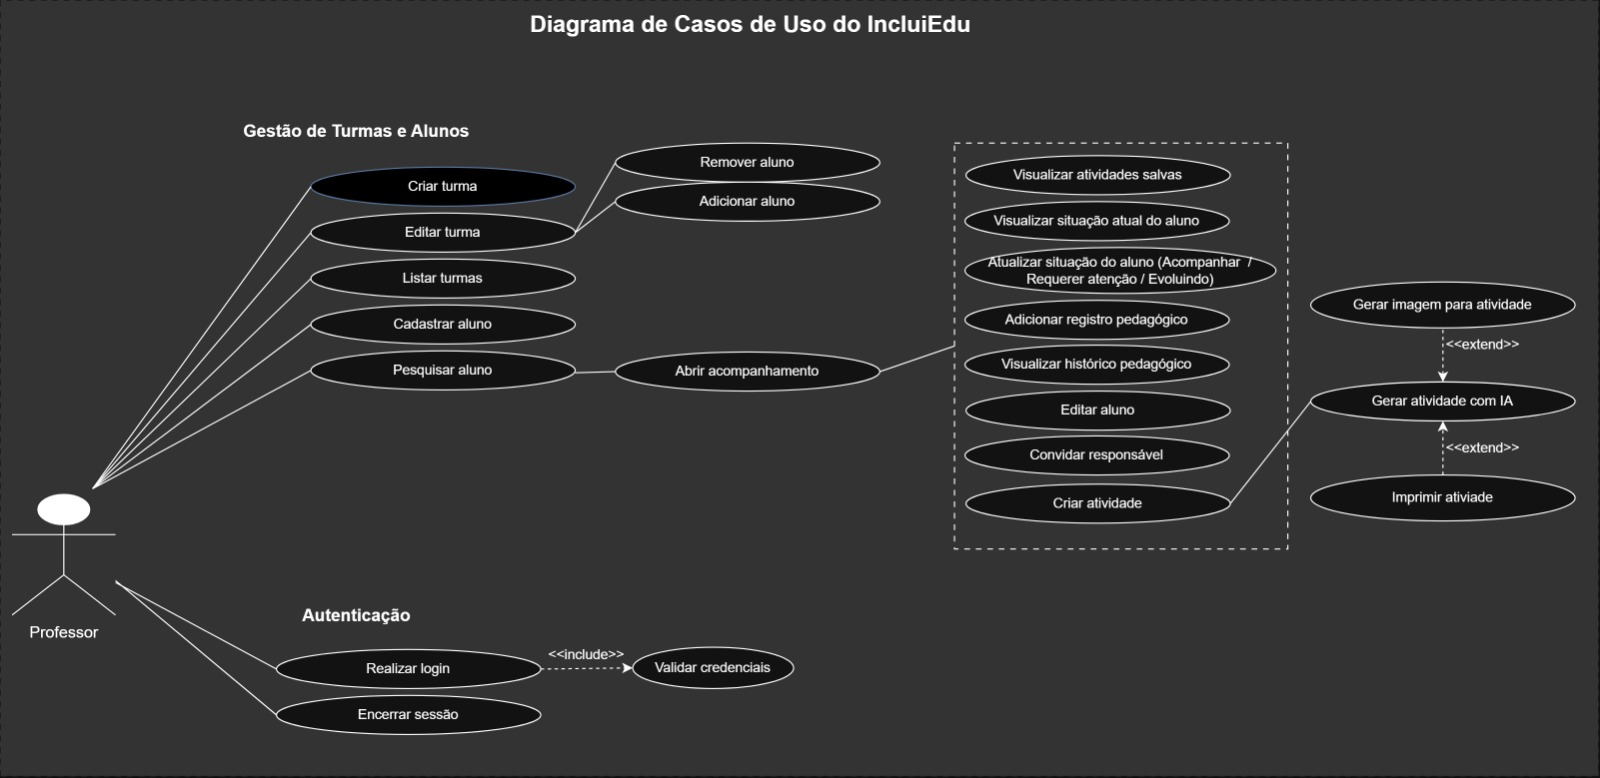
\includegraphics[width=0.9\textwidth]{04-figuras/casos_de_uso.jpeg}
    \fonte{Elaborado pelos autores (2026).}
\end{figure}

\subsection{DIAGRAMA DE CLASSES}
O diagrama de classes representa as principais entidades do sistema e seus relacionamentos. O professor está associado às turmas, que possuem alunos cadastrados. Cada aluno pode apresentar registros pedagógicos e atividades, permitindo a organização e a consulta das informações utilizadas no acompanhamento individual, conforme a Figura~\ref{fig:diagrama-classes}.

\begin{figure}[H]
    \centering
    \caption{Diagrama de Classes - IncluiEdu}
    \label{fig:diagrama-classes}
    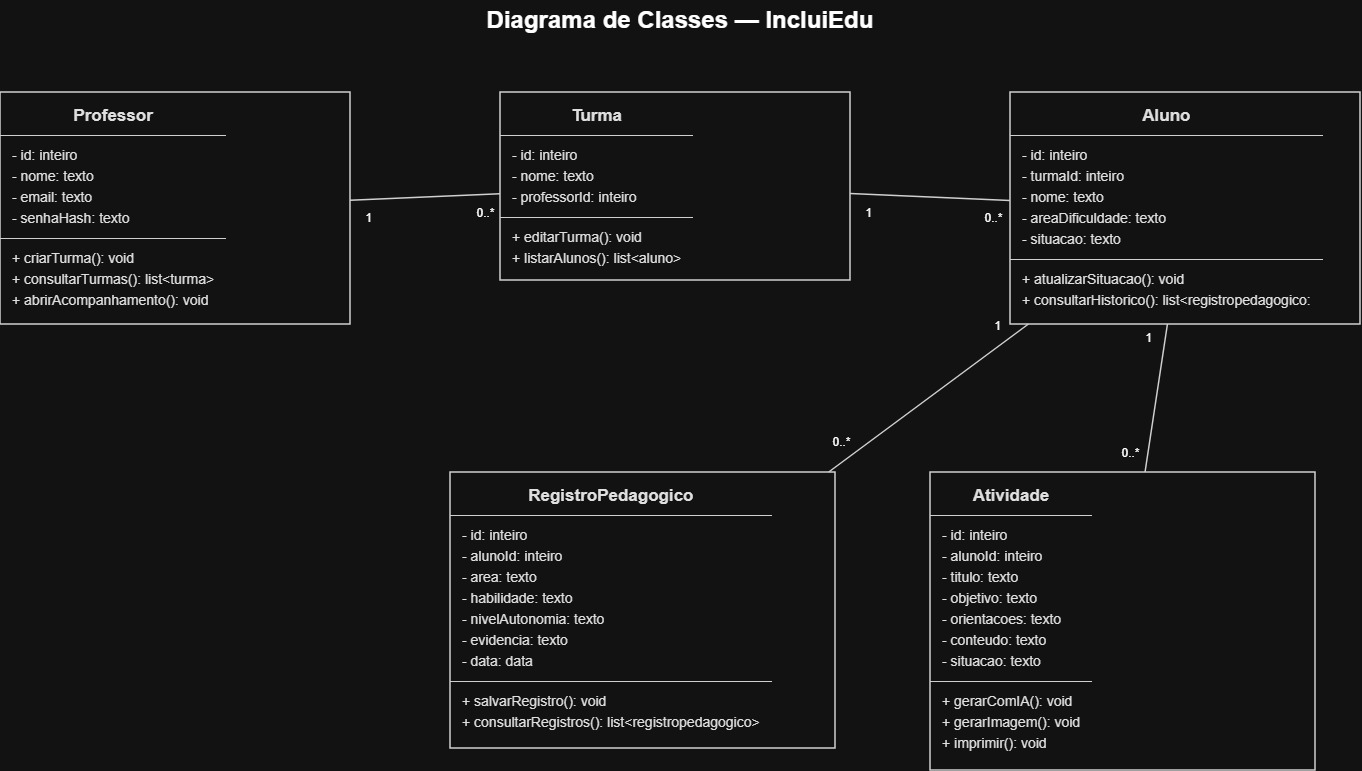
\includegraphics[width=0.9\textwidth]{04-figuras/diagrama_classes.jpeg}
    \fonte{Elaborado pelos autores (2026).}
\end{figure}

\subsection{MODELAGEM E IMPLEMENTAÇÃO DO BANCO DE DADOS}

A etapa local utilizou SQLite. Na versão atual, o Cloudflare D1 armazena dados em estrutura relacional \cite{cloudflare2026d1}. O modelo descrito compreende as entidades \texttt{users}, \texttt{classes}, \texttt{students}, \texttt{observations} e \texttt{activities}, relacionadas por chaves primárias e estrangeiras.

Um professor pode possuir diversas turmas; uma turma, diversos alunos; e cada aluno pode reunir observações e atividades ao longo do acompanhamento.

A estrutura do D1 é criada por migrações SQL, que documentam as tabelas e seus relacionamentos. As operações do backend utilizam instruções preparadas com parâmetros vinculados pelo método \texttt{.bind()}, evitando a concatenação direta dos valores recebidos em comandos SQL. O sistema verifica a vinculação dos registros ao professor autenticado antes de consultas ou alterações protegidas.

\begin{figure}[H]
    \centering
    \caption{Modelo do Banco de Dados - IncluiEdu}
    \label{fig:modelo-relacional}
    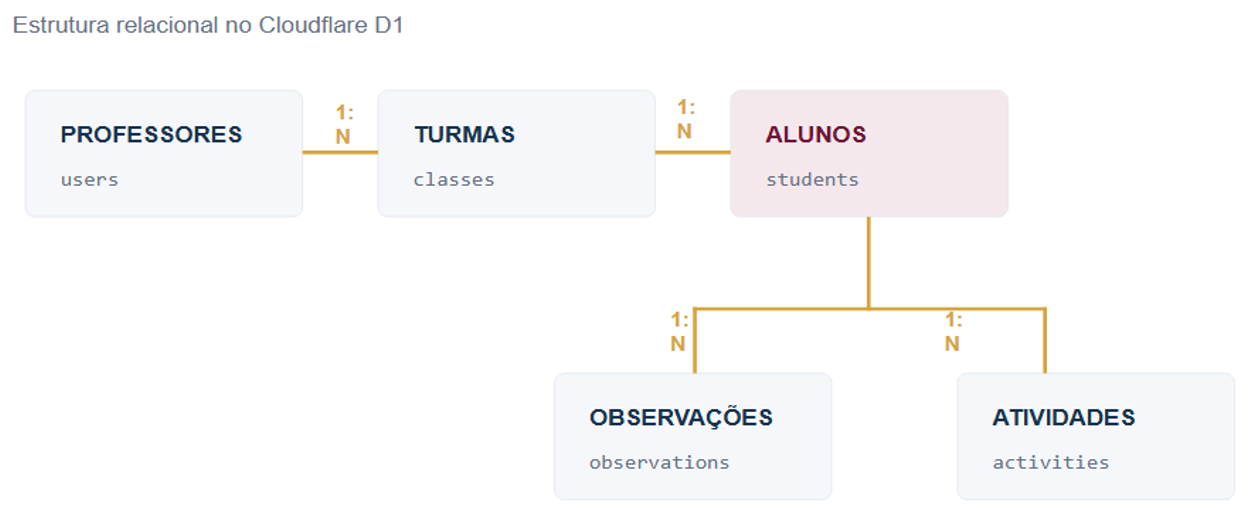
\includegraphics[width=0.9\textwidth]{04-figuras/modelo-relacional.png}
    \fonte{Elaborado pelos autores (2026).}
\end{figure}

\section{IMPLEMENTAÇÃO DO SISTEMA}

Na versão atual do IncluiEdu, a interface web apresenta as telas de cadastro, consulta e acompanhamento dos alunos. As ações realizadas pelo professor são enviadas à API por meio de requisições \texttt{fetch}, utilizando dados em formato JSON. O Cloudflare Worker recebe essas requisições, verifica a sessão e as permissões do usuário e realiza as operações necessárias no banco de dados D1. Em seguida, a resposta é enviada à interface, permitindo a atualização das informações apresentadas.

A autenticação utiliza derivação de senhas com PBKDF2, salt e SHA-256, evitando o armazenamento das senhas em texto simples. Após o login, o sistema cria uma sessão identificada por um cookie configurado com os atributos \texttt{HttpOnly}, \texttt{Secure} e \texttt{SameSite=Strict}. O backend também verifica se os registros acessados pertencem ao professor autenticado antes de permitir consultas ou alterações.

No acompanhamento pedagógico, cada registro reúne informações sobre o aluno, a área acompanhada, a habilidade observada, o nível de autonomia e as evidências registradas pelo professor. Esses dados são preservados no histórico pedagógico, permitindo acompanhar as observações realizadas ao longo do tempo. A situação do aluno também pode ser atualizada entre as opções \textit{Acompanhar}, \textit{Requer atenção} e \textit{Evoluindo}.

\section{TESTES E VALIDAÇÃO}

A verificação das funcionalidades do IncluiEdu foi realizada manualmente, por meio da interação com a aplicação. Os cenários de teste abrangem autenticação, organização de turmas, cadastro e consulta de alunos, observações pedagógicas, atualização da situação do aluno, geração de atividades e controle de acesso. Os procedimentos estão relacionados aos requisitos funcionais do sistema, conforme o Quadro~\ref{qua:testes}.

\begin{quadro}[htb]
\centering
\caption{Cenários de teste e resultados observados}
\label{qua:testes}
\small
\begin{tabular}{|p{2.5cm}|p{6cm}|p{5.5cm}|}
\hline
\textbf{Cenário} & \textbf{Procedimento realizado} & \textbf{Resultado} \\
\hline
Autenticação & Realização de login com credenciais válidas e inválidas. & O sistema permitiu o acesso com credenciais válidas e impediu a entrada com dados incorretos. \\
\hline
Turmas e alunos & Cadastro de turma e aluno, seleção de turma e pesquisa de aluno pelo nome. & As informações cadastradas foram exibidas corretamente, permitindo selecionar turmas e localizar alunos. \\
\hline
Acompanhamento & Abertura do acompanhamento individual de um aluno. & O sistema apresentou as informações do aluno, incluindo sua situação atual, registros pedagógicos e atividades salvas. \\
\hline
Registro pedagógico & Preenchimento dos campos de área, habilidade, nível de autonomia e evidência observada, seguido do salvamento. & O registro foi armazenado e disponibilizado para consulta no histórico pedagógico do aluno. \\
\hline
Situação do aluno & Alteração da situação entre \textit{Acompanhar}, \textit{Requer atenção} e \textit{Evoluindo}. & A situação foi atualizada e apresentada no perfil do aluno e no painel de acompanhamento. \\
\hline
Inteligência Artificial & Solicitação de uma atividade pedagógica personalizada por meio da IA. & O sistema apresentou uma atividade contendo título, objetivo, orientações e conteúdo pedagógico, identificada como rascunho para revisão. \\
\hline
Geração de imagem & Utilização da opção de gerar imagem para uma atividade produzida pela IA. & O sistema gerou uma imagem relacionada à atividade pedagógica solicitada, disponibilizando o resultado para utilização pelo professor. \\
\hline
Encerramento de sessão & Utilização da opção \textit{Sair} após autenticação. & A sessão foi encerrada, retornando o usuário à área de autenticação. \\
\hline
Controle de acesso & Tentativa de consultar registros de outro professor utilizando uma conta diferente. & O sistema impediu o acesso aos registros vinculados ao outro professor. \\
\hline
\end{tabular}
\fonte{Elaborado pelos autores (2026).}
\end{quadro}

Os testes manuais foram direcionados à observação do comportamento da versão atual da plataforma. A avaliação considerou os fluxos de utilização do professor e a comunicação entre interface, backend e serviços integrados.

\section{IMPLANTAÇÃO E REPRODUTIBILIDADE}

O IncluiEdu encontra-se publicado na plataforma Cloudflare, permitindo o acesso à aplicação por meio de um navegador web. A configuração do ambiente é organizada no arquivo \texttt{wrangler.jsonc}, que estabelece os vínculos necessários para o funcionamento dos serviços utilizados.

O código-fonte do projeto é mantido em um repositório no GitHub. Para reproduzir a aplicação em outro ambiente, é necessário obter os arquivos do projeto, configurar os serviços da Cloudflare, preparar o banco de dados D1 e realizar a publicação da aplicação.
        %
% Documento: Estrutura
%

\chapter{RESULTADOS}

A estrutura de acordo com a NBR-14724, compreende três elementos: pré-textuais, tex-tuais e pós-textuais.

\begin{figure}[H]
	\vspace*{0,2cm}
    \centering
    \caption{Ilustração da estrutura}
    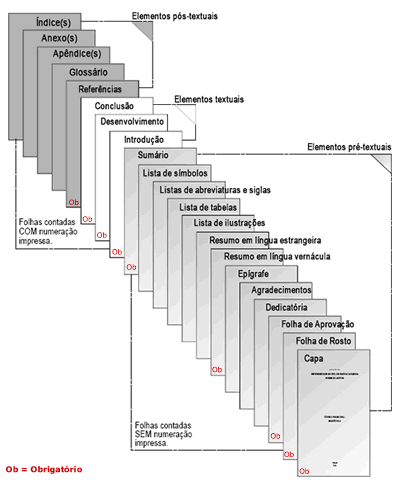
\includegraphics[width=0.6\textwidth]{./04-figuras/abnt}
    \label{fig:ilustfig2}
\end{figure}
\vspace*{-0,9cm}
{\raggedright \fonte{Disponível em: <https://www.intelligentsia.zip.net/estruturamonografia>. Acesso em: 15 ago. 2014.}}\\


\chapter{CONCLUSÃO}
Os Trabalhos de Conclusão de Curso (TCC) são documentos que
representam o resultado de estudo, devendo expressar conhecimento do assunto escolhido. Deve ser emanado da disciplina, módulo, estudo independente, curso, programa e outros ministrados. Deve ser feito sob a coordenação de um orientador.
A norma que determina os trabalhos com esse fim é a NBR 14724. Nesse documento será usada documentação o ABNTEX disponivel no site
\chapter{AGRADECIMENTOS}




    
        \include{./02-elementos-textuais/ambientes}  	
        %
% Documento: Citações
%

\section{Citações (ABNT NBR 10520)}

Esta seção apresenta exemplos práticos de citação conforme a ABNT NBR 10520.

\subsection{Citação direta curta (até 3 linhas)}
Deve permanecer no corpo do parágrafo, entre aspas duplas, com indicação de autor, ano e página:
\begin{flushleft}
\textit{Ex.:} De acordo com \citeonline[p.~249]{marshall1980}, ``não se pode discutir se o valor e os preços são governados pela utilidade ou pelo custo de produção''.
\end{flushleft}

Outras variações úteis:
\begin{itemize}
  \item Autor no texto + ano entre parênteses: \citeauthor{marshall1980} (\citeyear{marshall1980}) afirma que ``\ldots'' \cite[p.~249]{marshall1980}.
  \item Apenas referência entre parênteses: ``\ldots'' \cite[p.~249]{marshall1980}.
\end{itemize}

\subsection{Citação direta longa (mais de 3 linhas)}
Deve ir em bloco destacado, com recuo de 4\,cm da margem esquerda, fonte menor e sem aspas. 
No \texttt{abntex2}, use o ambiente \texttt{citacao}, que já aplica o padrão:
\begin{citacao}
Da mesma forma que não se pode afirmar se é a lâmina inferior ou superior de uma tesoura que corta uma folha de papel, também não se pode discutir se o valor e os preços são governados pela utilidade ou pelo custo de produção. (MARSHALL, 1980, p.~249)
\end{citacao}

\subsection{Citação indireta (paráfrase)}
Reproduz a ideia do autor com suas palavras. Página é opcional; recomenda-se quando ajuda o leitor.
\begin{flushleft}
\textit{Ex.:} A produção acadêmica sobre varejo no Brasil é desproporcional à relevância do segmento na economia \cite{angelo1993}.
\end{flushleft}
Variações:
\begin{itemize}
  \item \citeauthor{angelo1993} (\citeyear{angelo1993}) argumentam que \ldots
  \item Conforme apontado na literatura \cite{tanenbaum1995sistemas,de2017sistema}, \ldots
\end{itemize}

\subsection{Citação de citação (apud)}
Use somente quando o original não puder ser consultado. Indique o autor original, seguido de ``apud'' e do autor efetivamente consultado, com página.
\begin{flushleft}
\textit{Ex. no corpo do texto:} Enguita (apud \citeauthor{silva1991}, \citeyear{silva1991}, p.~21) chegou às mesmas conclusões.
\end{flushleft}

Também é possível registrar em nota de rodapé a fonte consultada:
\begin{flushleft}
\textit{Ex. com nota:} Enguita\footnote{Informação citada por \citeauthor{silva1991} (\citeyear{silva1991}, p.~21).} chegou às mesmas conclusões.
\end{flushleft}

\subsection{Comandos úteis (abntex2cite)}
\begin{itemize}
  \item \verb|\cite{chave}| → (AUTOR, ano)
  \item \verb|\citeonline{chave}| → AUTOR (ano)
  \item \verb|\citeauthor{chave}| → AUTOR
  \item \verb|\citeyear{chave}| → ano
  \item \verb|\cite[p.~10]{chave}| → (AUTOR, ano, p.~10)
\end{itemize}

\subsection{Observações finais}
\begin{itemize}
  \item Para siglas: escreva por extenso na primeira ocorrência, seguidas da sigla: Associação Brasileira do Trabalhador (ABT).
  \item As referências completas devem aparecer na lista de referências ao final do trabalho.
\end{itemize}

  	
    
\end{OnehalfSpacing}

    % Elementos pós-textuais
    \postextual
    %
% Documento: Referências Bibliográficas
%

\bibliography{referencias}    % Geração automática das referências por meio do arquivo 'referencias.bib'
       

\end{document}
